\documentclass[english,man, mask]{apa6}

\usepackage{amssymb,amsmath}
\usepackage{ifxetex,ifluatex}
\usepackage{fixltx2e} % provides \textsubscript
\ifnum 0\ifxetex 1\fi\ifluatex 1\fi=0 % if pdftex
  \usepackage[T1]{fontenc}
  \usepackage[utf8]{inputenc}
\else % if luatex or xelatex
  \ifxetex
    \usepackage{mathspec}
    \usepackage{xltxtra,xunicode}
  \else
    \usepackage{fontspec}
  \fi
  \defaultfontfeatures{Mapping=tex-text,Scale=MatchLowercase}
  \newcommand{\euro}{€}
\fi
% use upquote if available, for straight quotes in verbatim environments
\IfFileExists{upquote.sty}{\usepackage{upquote}}{}
% use microtype if available
\IfFileExists{microtype.sty}{\usepackage{microtype}}{}

% Table formatting
\usepackage{longtable, booktabs}
\usepackage{lscape}
% \usepackage[counterclockwise]{rotating}   % Landscape page setup for large tables
\usepackage{multirow}		% Table styling
\usepackage{tabularx}		% Control Column width
\usepackage[flushleft]{threeparttable}	% Allows for three part tables with a specified notes section
\usepackage{threeparttablex}            % Lets threeparttable work with longtable

% Create new environments so endfloat can handle them
% \newenvironment{ltable}
%   {\begin{landscape}\begin{center}\begin{threeparttable}}
%   {\end{threeparttable}\end{center}\end{landscape}}

\newenvironment{lltable}
  {\begin{landscape}\begin{center}\begin{ThreePartTable}}
  {\end{ThreePartTable}\end{center}\end{landscape}}

  \usepackage{ifthen} % Only add declarations when endfloat package is loaded
  \ifthenelse{\equal{\string man, mask}{\string man}}{%
   \DeclareDelayedFloatFlavor{ThreePartTable}{table} % Make endfloat play with longtable
   % \DeclareDelayedFloatFlavor{ltable}{table} % Make endfloat play with lscape
   \DeclareDelayedFloatFlavor{lltable}{table} % Make endfloat play with lscape & longtable
  }{}%



% The following enables adjusting longtable caption width to table width
% Solution found at http://golatex.de/longtable-mit-caption-so-breit-wie-die-tabelle-t15767.html
\makeatletter
\newcommand\LastLTentrywidth{1em}
\newlength\longtablewidth
\setlength{\longtablewidth}{1in}
\newcommand\getlongtablewidth{%
 \begingroup
  \ifcsname LT@\roman{LT@tables}\endcsname
  \global\longtablewidth=0pt
  \renewcommand\LT@entry[2]{\global\advance\longtablewidth by ##2\relax\gdef\LastLTentrywidth{##2}}%
  \@nameuse{LT@\roman{LT@tables}}%
  \fi
\endgroup}


  \usepackage{graphicx}
  \makeatletter
  \def\maxwidth{\ifdim\Gin@nat@width>\linewidth\linewidth\else\Gin@nat@width\fi}
  \def\maxheight{\ifdim\Gin@nat@height>\textheight\textheight\else\Gin@nat@height\fi}
  \makeatother
  % Scale images if necessary, so that they will not overflow the page
  % margins by default, and it is still possible to overwrite the defaults
  % using explicit options in \includegraphics[width, height, ...]{}
  \setkeys{Gin}{width=\maxwidth,height=\maxheight,keepaspectratio}
\ifxetex
  \usepackage[setpagesize=false, % page size defined by xetex
              unicode=false, % unicode breaks when used with xetex
              xetex]{hyperref}
\else
  \usepackage[unicode=true]{hyperref}
\fi
\hypersetup{breaklinks=true,
            pdfauthor={},
            pdftitle={A Meta-Analysis of Expressive Writing on Quality of Life, Posttraumatic Growth, and Posttraumatic Stress},
            colorlinks=true,
            citecolor=blue,
            urlcolor=blue,
            linkcolor=black,
            pdfborder={0 0 0}}
\urlstyle{same}  % don't use monospace font for urls

\setlength{\parindent}{0pt}
%\setlength{\parskip}{0pt plus 0pt minus 0pt}

\setlength{\emergencystretch}{3em}  % prevent overfull lines

\ifxetex
  \usepackage{polyglossia}
  \setmainlanguage{}
\else
  \usepackage[english]{babel}
\fi

% Manuscript styling
\captionsetup{font=singlespacing,justification=justified}
\usepackage{csquotes}
\usepackage{upgreek}

 % Line numbering
  \usepackage{lineno}
  \linenumbers


\usepackage{tikz} % Variable definition to generate author note

% fix for \tightlist problem in pandoc 1.14
\providecommand{\tightlist}{%
  \setlength{\itemsep}{0pt}\setlength{\parskip}{0pt}}

% Essential manuscript parts
  \title{A Meta-Analysis of Expressive Writing on Quality of Life, Posttraumatic
Growth, and Posttraumatic Stress}

  \shorttitle{Expressive Writing}


  \author{Jeffrey M. Pavlacic\textsuperscript{1}, Erin M. Buchanan\textsuperscript{2}, Nicholas P. Maxwell\textsuperscript{2}, Tabetha G. Hopke\textsuperscript{2}, \& Stefan E. Schulenberg\textsuperscript{1}}

  \def\affdep{{"", "", "", "", ""}}%
  \def\affcity{{"", "", "", "", ""}}%

  \affiliation{
    \vspace{0.5cm}
          \textsuperscript{1} University of Mississippi\\
          \textsuperscript{2} Missouri State University  }

  \authornote{
    \newcounter{author}
    Jeffrey M. Pavlacic is a doctoral candidate at the University of
    Mississippi and a member of the University of Mississippi
    Clinical-Disaster Research Center (UM-CDRC). Erin M. Buchanan is an
    Associate Professor of Psychology at Missouri State University. Nicholas
    P. Maxwell and Tabetha G. Hopke are master's degree candidates at
    Missouri State University. Stefan E. Schulenberg is a Professor of
    Psychology at the University of Mississippi and director of the UM-CDRC.

                      Correspondence concerning this article should be addressed to Jeffrey M. Pavlacic, 205 Peabody Hall, University, MS 38655. E-mail: \href{mailto:jpavlaci@go.olemiss.edu}{\nolinkurl{jpavlaci@go.olemiss.edu}}
                                                        }


  \abstract{Emotional expression has been shown to be beneficial for promoting both
positive psychological and physical health outcomes. Unfortunately,
inhibiting emotions can lead to impairments in physical and
psychological health. James Pennebaker showed that expressive writing is
an effective form of emotional expression, and he and others have used
expressive writing as an experimental manipulation to gauge its efficacy
in treating a wide variety of health-related and psychological outcomes.
While many studies have been conducted that examine the efficacy of
expressive writing across such outcomes, a considerable amount of these
studies tend to neglect necessary considerations such as power and
meaningfulness of respective effect sizes. Six previous meta-analyses
have been conducted that examine expressive writing's effect on
psychological outcomes. However, these studies focus on the experimental
versus control group effect size. Thus, our meta-analysis sought to
examine the efficacy of an expressive writing task on only the
experimental conditions in studies measuring posttraumatic growth,
posttraumatic stress, and quality of life using random effects models.
Results indicated a small overall effect size for posttraumatic stress
and negligible to small effect sizes for posttraumatic growth and
quality of life. Implications for future research design and
interpretation of published research are discussed.}
  \keywords{meta-analysis, positive psychology, expressive writing \\

    
  }





\usepackage{amsthm}
\newtheorem{theorem}{Theorem}
\newtheorem{lemma}{Lemma}
\theoremstyle{definition}
\newtheorem{definition}{Definition}
\newtheorem{corollary}{Corollary}
\newtheorem{proposition}{Proposition}
\theoremstyle{definition}
\newtheorem{example}{Example}
\theoremstyle{definition}
\newtheorem{exercise}{Exercise}
\theoremstyle{remark}
\newtheorem*{remark}{Remark}
\newtheorem*{solution}{Solution}
\begin{document}

\maketitle

\setcounter{secnumdepth}{0}



\subsection{Emotional Expression}\label{emotional-expression}

Emotional expression relating to negative emotions or trauma has been
shown to enhance both mental and physical health outcomes (Esterling,
Antoni, Kumar, \& Schneiderman, 1990; Fawzy et al., 1993; Lieberman \&
Goldstein, 2006; Rachman, 1980; Scheff, 1979). For example, the
disclosure of traumatic or stressful events has been shown to reduce
stress and lead to positive health outcomes in those with diabetes
(Bodor, 2002) and breast cancer (Stanton et al., 2002), among others.
Inhibiting repressive thoughts or emotions, rather, may be detrimental
to both physical and psychological health (H. S. Goldstein, Edelberg,
Meier, \& Davis, 1988; Gross \& Levenson, 1997; Larson \& Chastain,
1990). While some studies suggest that emotional expression in the form
of \enquote{truth telling} may cause psychological harm to individuals
(Brounéus, 2010), the literature presents a plethora of evidence
confirming the negative effects of a lack of emotional expression, such
as social concerns, overall psychological dysfunction, and lack of
value-congruent behaviors (Frankl, 1959; Pennebaker, 1989; Pennebaker \&
Beall, 1986; Schulenberg, Hutzell, Nassif, \& Rogina, 2008; Wilson \&
DuFrene, 2009). These resulting negative outcomes may lead to
detrimental effects on health (Pennebaker \& Beall, 1986). Individuals
having experienced a traumatic or stressful life event are significantly
more likely to repress thoughts and feelings about their experience
compared to individuals who have not experienced such events, thereby
subjecting them to potential negative outcomes caused by a lack of
emotional expression (Bodor, 2002).

\subsection{Expressive Writing as Effective Emotional
Expression}\label{expressive-writing-as-effective-emotional-expression}

Pennebaker and Beall (1986) first showed that emotional expression can
be both experimentally manipulated and have positive benefits to
participants. In their seminal study, they randomly assigned
participants to several writing groups, including writing about a
\enquote{stressful or traumatic} life event or a neutral event. As such,
the content of the writing likely varies widely based on the contextual
factors (e.g.~topic, setting, sample, health concern). The group that
disclosed both regarding their trauma and the emotions surrounding said
trauma later showed a reduction in health visits. Pennebaker has
replicated the use of expressive writing across a number of studies
ranging from improved health (Pennebaker, Colder, \& Sharp, 1990;
Pennebaker, Kiecolt-Glaser, \& Glaser, 1988) to improvements in school
(Pennebaker \& Francis, 1996) and work (Francis \& Pennebaker, 1992).
Others have expanded this work to show positive effects on mood
(Schoutrop, Lange, Hanewald, Davidovich, \& Salomon, 2002) and asthma
(Smyth, Stone, Hurewitz, \& Kaell, 1999); however, several controlled
studies have shown to not replicate (Harris, Thoresen, Humphreys, \&
Faul, 2005) or null effects (Gidron, Peri, Connolly, \& Shalev, 1996;
Walker, Nail, \& Croyle, 1999).

The idea that a brief, controlled writing task can have numerous
positive health and psychological benefits can certainly be
controversial, given the existing literature. For example, Henry,
Schlegel, Talley, Molix, and Bettencourt (2010) found that expressive
writing only benefited a rural population for those individuals
surviving breast cancer on physical and psychological health outcomes,
while Lancaster, Klein, and Heifner (2015) found no significant evidence
that expressive writing can be considered an effective approach in
measuring posttraumatic growth. Additionally and as mentioned, Brounéus
(2010) found that \enquote{truth telling} caused harm to individuals in
a forensic setting. Regardless, the concept remains interesting due to
the nature and inexpensive implementation of expressive writing. Many
individuals who have experienced traumatic events do not wish to
disclose their feelings regarding the events with others. Additionally,
those who do not meet diagnostic criteria (e.g.~subclinical symptoms)
are sometimes neglected despite probable suffering (Wilson \& DuFrene,
2009). However, by utilizing expressive writing as a personal method of
treatment, individuals are able to effectively express their emotions
while avoiding talking to another individual or clinician about the
traumatic event (Smyth, 1998). Pennebaker (1993) found that experimental
conditions assigned to participate in an expressive writing task
generally report more positive changes than those in control conditions.
Some controversy has been observed over whether or not writing about a
formerly disclosed event is more effective than writing about an
undisclosed event. M. A. Greenberg and Stone (1992) conducted an
experiment where they separated participants into three groups: writing
about a formerly disclosed trauma, writing about an undisclosed trauma,
and a control group. They found no difference between groups in
efficacy. However, they did find that those who disclosed more severe
traumas reportedly experienced fewer physical symptoms at follow up,
which suggests that the type of trauma revealed can play a significant
impact on symptom reduction and physical health. A review of current
meta-analyses is presented in a subsequent section.

\subsection{Possible Mechanisms Underlying Expressive Writing
Efficacy}\label{possible-mechanisms-underlying-expressive-writing-efficacy}

In order to understand why expressive writing is considered to be
efficacious, one must examine the cognitive, social, and behavioral
processes by which it allows information processing. Pennebaker et al.
(1990) discovered that individuals who benefited from expressive writing
attributed their success from the writing task to a renewed sense of
understanding. Further, Pennebaker (1993) conducted a textual analysis
on expressive writing content and found that those who were more
successful during the task used causation words. Pennebaker considered
expressive writing as a way for individuals to effectively process the
event in their minds, which may explain the aforementioned renewed sense
of understand and excess of causation-oriented words. Aside from
theories related to cognitive-processing and inhibition, there are a
number of other theories related to emotional disclosure that warrant
explanation. The first is the social integration model (Pennebaker \&
Graybeal, 2001). This model suggests emotional disclosure can have a
positive impact on how people interact in their environment. This
increased environmental interaction has been shown to have positive
benefits on health (Frattaroli, 2006). Second, expressive writing
parallels exposure therapy for phobias and posttraumatic stress
disorder, which suggests that repeatedly exposing oneself to the fear or
trauma can reduce the negative emotions associated with that fear or
trauma (Meshberg-Cohen, Svikis, \& McMahon, 2014). Given that exposure
therapy has been shown to be effective for reducing symptoms of
posttraumatic stress (PTS; Sloan, Marx, \& Epstein, 2005), one would
expect individuals in these studies to experience a reduction in PTS
symptoms after taking part in an expressive writing task. Third, Wilson
and DuFrene (2009) discussed how the nonjudgmental acceptance of
emotions leads to positive health benefits by promoting value-congruent
behavior, one of the main facets of Functional Contextualism theory and
Logotherapy (Frankl, 1959; Schulenberg et al., 2008). Indeed, emotional
expression in the form of expressive writing could be considered a form
of nonjudgmental acceptance, although it may not necessarily lead to
behavior change. Engaging in value-congruent behavior in the presence of
inevitable emotional experiences is also the most crucial tenet in
Logotherapy. Finally, a recently proposed theory that may help explain
positive outcomes is referred to as a distance percpetive (Kross and
Ayduk (2011)). This theory posits that, when individuals adopt a
psychologically distanced perspective, they are better able to better
understand their life situation. In sum, it seems likely that there are
multiple underlying mechanisms that account for the beneficial outcomes
associated with expressive writing described below. Indeed, the wide
range of theroetical perspectives provide further evidence which
suggests that expressive writing is applicable in a variety of contexts.
Previously conducted meta-analyses, however, present varying results.

\subsection{Meta-Analytic Techniques}\label{meta-analytic-techniques}

Meta-analyses allow researchers the opportunity to collectively examine
the efficacy of different psychological interventions/tasks on outcome
variables (Borenstein, Hedges, \& Rothstein, 2007; Glass, 1976; Hedges,
1982). Although many studies produced positive outcomes associated with
expressive writing, some of these studies tend to neglect important
questions, the most important of which is whether or not the effect
sizes are meaningful (Smyth, 1998). Meta-analyses are a technique that
allows researchers to pool studies to examine an overall, weighted,
population effect (Borenstein et al., 2007). Several meta-analyses of
expressive writing and emotional expression have been explored that
warrant considerable explanation: Smyth (1998), Frisina, Borod, and
Lepore (2004), Frattaroli (2006), Reinhold, Bürkner, and Holling (2018),
Van Emmerik, Reijntjes, and Kamphuis (2013) and Mogk, Otte,
Reinhold-Hurley, and Kröner-Herwig (2006). These meta-analyses have laid
a foundation for exploring the effects of writing on psychological
outcomes. The meta-analyses described sequentially below focused on
experimental versus control group effect sizes or \emph{p}-values,
rather than emphasizing change for an writing group. This focus is
likely because of the analyses provided in these publications,
especially when using randomized controlled trial research designs.
While this design is the gold standard for medicine, the current
meta-analysis sought to examine the magnitude of change for participants
who experienced an expressive writing task. For example, a comparison
group may increase their quality of life scores by two points in a
controlled study, while the experimental group increases their quality
of life scores by four points; thus, creating a significant difference
in change between the two groups. This information is valuable, but it
does not tell the reader the magnitude of the change for the writing
group, wherein four points might only be a small effect when examined
within the group who received the writing task. This study will focus on
changes across time for groups who received the expressive writing task
to determine what size of effects one might expect given a specific
measurement schedule (i.e., one to three months, three months to six
months, etc.). Additionally, the current meta-analysis will examine the
change in effects across measurement time to determine whether or not
effects decrease over time.

Smyth (1998) conducted the seminal meta-analysis regarding the efficacy
of expressive writing. They included studies utilizing an expressive
writing group and control group (neutral topic). This particular
analysis examined the efficacy of expressive writing on psychological
well-being, general health, and physical functioning. In sum, 13
studies/effect sizes were included, and the authors found an overall
medium effect size, \emph{d} = 0.47, for the experimental group compared
to the control group. A later meta-analysis conducted by Frisina et al.
(2004) expanded these analyses. They only included studies utilizing
clinical samples and employing the paradigm adapted by Pennebaker and
Beall (1986). This meta-analysis included 9 studies in total and found
an effect size of \emph{d} = .19 for health-related outcomes and
\emph{d} = .07 for psychological outcomes. The next meta-analysis
regarding expressive writing was conducted by Mogk et al. (2006) and
aimed to update the state of the literature on expressive writing.
Similar to previously-conducted analysis, they included studies
employing Pennebaker's paradigm on experimental and control groups.
Additionally, they only included studies with a 4-week follow up that
included at least 10 participants. In sum, 30 studies met their
criteria. They found nonsignificant effects on somatic and psychological
health outcomes and concluded that expressive wrting does not benefit
health. These findings corroboate those from Frisina et al. (2004).
Frattaroli (2006) conducted perhaps the most notable meta-analysis to
data examining the efficacy of emotional disclosure on the folliwing
constructs using only randomized and control conditions: psychological
health, physiological functioning, reported health, health behaviors,
and general functioning/life outcomes. Additionally, their meta-analysis
employed random effects models. Prior meta-analysis employed fixed
effects models, which assume that all studies assess the same
\enquote{true} population effect size, which may be an untenable
assumption across different assessment and populations (Borenstein et
al., 2007). Random effects models, rather, estimate the mean of a
proposed distribution of population effect sizes, which may vary by
subject type or research design. They included a wide range of studies,
\emph{N} = 146. Individual studies were again collapsed into one
publication effect size, although these effects were also examined
separately by health outcome. Overall, Frattaroli (2006) found a
weighted \emph{r} effect size of .08 for all outcomes combined, which
would be considered small. Additionally, they examined potential
moderators and found larger effect sizes for the following samples:
those with physical health problems, those with a history of having
experienced traumatic or stressful events, samples not including college
students, samples where expressive writing tasks were conducted at home
and in private settings, paid participants, more male participants, and
fewer participants (see Frattaroli, 2006 for a complete list of
moderators). A recent analysis conducted by Van Emmerik et al. (2013)
employing Pennebaker's paradigm found included 6 eligible studies that
compared treatment to control groups. In regards to inclusion criteria,
they included studies where participants had a diagnosis of Acute Stress
Disorder (ASD) or Posttraumatic Stress Disorder (PTSD). They found that
those who participated in the expressive writing group experienced
short-term reductions in PTS and depressive symptoms. combined Hedges'
\emph{g} = .81. The most recently published meta-analysis was conducted
by Reinhold et al. (2018) and examined the effects of expressive writing
on depression by randomizing participants to conditions (expressive
writing vs.~control). They included 39 randomized controlled trials and
excluded individuals with diagnoses of PTSD. This study did not support
utilizing expressive writing for depression outcome measures. Further,
they found that expressive writing did not yield any type of long-term
effect on depression outcomes.

\subsection{Posttraumatic Stress}\label{posttraumatic-stress}

Posttraumatic Stress Disorder (PTSD) is a disorder involving
re-experiencing thoughts or experiences after a traumatic event or
experience. This generates a context where individuals are prone to
affect-related deficiencies and maladaptive behaviors (American
Psychiatric Association, 2013). DSM-5 criteria are based on 20 symptoms
structured into four different subsets in those having experienced a
traumatic event. These subsets are as follows: re-experiencing,
avoidance, negative alterations in cognition and mood, and increased
arousal (Crespo \& Gomez, 2016). While the renewed DSM-5 criteria are
commonly employed, the current meta-analysis considers studies using
DSM-IV criteria. DSM-IV criteria are similar and include the following:
exposure to a traumatic event, re-experiencing (intrusion), avoidance,
and increased arousal (American Psychiatric Association, 2013). Further,
the studies employed in the current meta-analysis are divided according
to these subsets (arousal, intrusion, and avoidance). PTSD affects a
wide variety of groups, a few of which are sexual assault survivors
(Klump, 2008), Iraq and Afghanistan war veterans (Gentes et al., 2014),
and those exposed to natural disasters (Wang et al., 2000). Research
conducted on the efficacy of expressive writing on PTSD symptoms has
been less successful and shows outcomes that are not as effective as
other studies. While PTSD symptoms decreased after a written emotional
disclosure task, this decrease was not significantly different than a
control group change (Sloan, Marx, \& Greenberg, 2011). However, other
studies show contradicting results. For example, Sloan, Marx, Epstein,
and Lexington (2007) examined individuals with at least moderate PTSD
symptom severity and found that individuals assigned to an emotional
expression writing condition reported fewer PTSD and depression symptoms
during follow up. Additionally, in 2012, Sloan, Marx, Bovin, Feinstein,
and Gallagher (2012) adapted their writing protocol to focus primarily
on the emotions, meaning, and \enquote{hot spots} associated with the
trauma. They referred to this as the written exposure therapy (WET)
protocol, distinguishable from that adapted by Pennebaker and Beall
(1986).

Di Blasio et al. (2015) recruited women who had just given birth and
assessed them a few days after experiencing childbirth along with a
three-month follow-up. Results showed that women who had participated in
the expressive writing task had lower depression and posttraumatic
stress symptoms than the group assigned to a neutral writing condition.
Additionally, regression models showed that expressive writing was
significantly linked to a reduction of PTSD symptoms across different
dimensional levels of symptom severity. Contradicting the work conducted
by Sloan et al. (2011), these results suggest that expressive writing
may be an effective tool for women managing postpartum distress.
However, it is important to note that only 20 of the 113 women recruited
for this study qualified for a diagnosis of PTSD. This limitation
suggests that those with moderate distress could perhaps benefit more
from an expressive writing task than those diagnosed with or meeting the
qualifications for PTSD. It may also explain the differences in results
between the two studies, as Sloan et al. (2011) found that those with a
clinical diagnosis of PTSD did not respond to an emotional disclosure
writing task. Di Blasio et al. (2015) found that those who reported mild
symptomology better responded to the task than those meeting the
criteria for a diagnosis of PTSD. Perhaps it is more advantageous to
examine effect sizes separately in with diagnoses of PTSD and
subclinical symptoms.

\subsection{Posttraumatic Growth}\label{posttraumatic-growth}

While the literature mostly discusses potentially harmful outcomes to
traumatic events such as emotional distress, traumatic events also
provide opportunities for personal growth (Aslam \& Kamal, 2013).
Traumatic events, either natural or human-inflicted, can lead to
positive outcomes by allowing the individual to take a different
perspective (Cobb, Tedeschi, Calhoun, \& Cann, 2006; Taku, Calhoun,
Cann, \& Tedeschi, 2008). The relationship between positive growth after
a traumatic event and symptom reduction is unclear, as it is a complex
process. Thus, it is necessary to examine how expressive writing might
influence each variable separately, which is one of the key goals of
this meta-analysis (Slavin-Spenny, Cohen, Oberleitner, \& Lumley, 2011).
Models receiving empirical support within the last decade suggest that
traumatic events offer opportunities for both negative and positive
experiences (Tedeschi \& Calhoun, 1995; Weiss, 2002). Posttraumatic
Growth (PTG) is a positive experience after a traumatic event (Aslam \&
Kamal, 2013; Yilmaz \& Zara, 2016). Specifically, PTG is classified as
broad cognitive benefits that are seen after a traumatic experience.
These benefits can be categorized into building closer relationships,
examining new possibilities, appreciating life, recognizing personal
strengths, and undergoing spiritual changes. (Dursun, Steger, Bentele,
\& Schulenberg, 2016; Tedeschi \& Calhoun, 2004).

PTG is associated with a variety of desired outcomes (Dursun et al.,
2016). PTG has been studied in those experiencing natural disasters,
war, and other harms such as sexual assault. Finally, PTG has been
studied in those experiencing medical diagnoses such as different types
of cancer and diseases. Although the relationship between PTG and
symptom reduction is not yet fully understood, perhaps expressive
writing allows the individual to fully comprehend the event. Pennebaker
and Graybeal (2001) speculated that expressive writing allows an
individual to feel more connected with his or her surroundings. Although
this speculation does not directly explain positive outcomes after an
expressive writing task, perhaps individuals gain a better appreciation
for life after gaining a better sense of connectedness with that
individual's surroundings.

\subsection{Quality of Life}\label{quality-of-life}

Quality of Life (QOL), according to Theofilou (2013) is an evaluation of
the \enquote{goodness} that an individual experiences, separated into
domains of reactions to life events, disposition, life fulfillment, and
satisfaction with life experiences. More generally, QOL refers to an
individual's attitude towards the target life situation (Costanza et
al., 2007), delineated into objective and subjective components.
Objectively, QOL refers to components outside of an individual and
measurable by others, while subjective QOL is an individual's assessment
of his or her own experiences (Costanza et al., 2007). The current
meta-analysis will focus solely on the subjective components of QOL, as
it is obtainable through questionnaires. Pennebaker and Graybeal (2001)
suggested that expressive writing allows one to feel more connected with
their surroundings. Further, they explain that expressive writing allows
people to see things in a different way and better understand
themselves. By understanding a traumatic or stressful event, one is said
to see things differently and perhaps look at the situation with a more
positive mindset. The changes that occur after expressive writing may
also allow one to find meaning in the traumatic event, thereby
increasing the QOL of that individual (Frankl, 1959). Higher QOL may be
considered a type of PTG, which is why the current meta-analysis sought
to examine the efficacy of studies utilizing expressive writing to
improve QOL and PTG in the same study.

\subsection{Current Meta-Analysis}\label{current-meta-analysis}

The purpose of the current meta-analysis is to examine studies employing
expressive writing procedures using Pennebaker's paradigm on variables
relevant to the field of positive psychology (PTG and QOL) and PTS, with
effect sizes separated by those having and not having a diagnosis of
PTSD. Based on recently published literature regarding efficacy of
expressive writing for different levels of PTSD symptoms, this is an
important facet to consider, (Reinhold et al., 2018). Additionally, no
meta-analysis has been conducted that examines the efficacy of
expressive writing on positive outcome variables such as PTG and QOL.
The meta-analyses described sequentially above focused on experimental
versus control group effect sizes or \emph{p}-values, rather than
emphasizing change for the expressive writing group. This focus is
likely because of the analyses provided in these publications,
especially when using randomized controlled trial research designs.
While this design is the gold standard for medicine, the current
meta-analysis sought to examine the magnitude of change for participants
who experienced an expressive writing task. For example, a comparison
group may increase their quality of life scores by two points in a
controlled study, while the experimental group increases their quality
of life scores by four points; thus, creating a significant difference
in change between the two groups. This information is valuable, but it
does not tell the reader the magnitude of the change for the writing
group, wherein four points might only be a small effect when examined
within the group who received the writing task. This study will focus on
changes across time for groups who received the expressive writing task
to determine what size of effects one might expect given a specific
measurement schedule (i.e., one to three months, three months to six
months, etc.). This analysis should present researchers with a renewed
examination of the efficacy of expressive writing on the aforementioned
variables using newer meta-analytic techniques. Newer methods of
meta-analysis, including \emph{p}-curve (Simonsohn, Nelson, \& Simmons,
2014; Simonsohn, Simmons, \& Nelson, 2015), \emph{p}-uniform (Aert,
Wicherts, \& Van Assen, 2016), PET-PEESE (Stanley \& Doucouliagos,
2014), selection models (Vevea \& Hedges, 1995), and trim and fill
methods (Carter \& McCullough, 2014) allow for better estimation of
meta-analytic effect sizes. These analyses would be best performed by
examining each potential effect separately, rather than averaging
effects of each publication into one study effect size (a common trend
in the previously mentioned meta-analysis). In addition to an estimate
of overall effect sizes using updated techniques, the current
meta-analysis estimates power for effects on writing groups, as research
has shown a consistent underpowering of psychological studies, combined
with a misunderstanding of the sample size needed for adequately
powering one's work (Bakker, Hartgerink, Wicherts, \& Maas, 2016).

\section{Method}\label{method}

\subsection{Data Collection}\label{data-collection}

Studies were collected through online databases, such as PsycINFO and
Google Scholar, using the following search terms and their combinations:
\emph{Posttraumatic Growth, PTG, Quality of Life, QOL, Posttraumatic
Stress, PTS, Expressive Writing, Emotional Disclosure, Narrative
Writing}. Within these articles, the change in outcome variables (PTS,
PTG, QOL) from pre- to post-test was the dependent variable of interest.
Generally, groups were separated into an experimental and control group
and then examined at different time points. For purposes of this
meta-analysis, only participants assigned to the experimental condition
were examined due to having received the expressive writing task. If a
study included multiple assessment time points, then these measurements
were examined sequentially (i.e., time 1 to time 2, time 2 to time 3) to
determine change across time for the dependent variable.

220 citations focusing on PTS, PTG, and QOL were identified through the
literature search and previous meta-analyses. After screening these
studies, forty-five articles were retained for containing the
appropriate information for this meta-analysis. A complete list of
excluded articles can be found at \url{https://osf.io/4mjqt}, along with
reasons why they were excluded. Generally, studies were included if they
utilized the expressive writing paradigm adapted by Pennebaker and Beall
(1986), included relevant numbers to compute an effect size, and
included the relevant outcome variables. After having two reviewers
independent code articles, 202 effect sizes were calculated from the
forty-five studies. On average, each study represented \emph{M} = 4.49
(\emph{SD} = 3.50) effects, ranging from 1 to 16 effects. 144 effects
were calculated for PTS, 21 for PTG, and 37 for QOL.

\subsection{Calculations for Effect Size, Variance, and Confidence
Intervals}\label{calculations-for-effect-size-variance-and-confidence-intervals}

For our purposes, we used Cohen's (1988) standards for nomenclature for
small (0.20), medium (0.50), and large (0.80) \emph{d} values, although
it is important to note that Cohen himself suggested that these values
should be based on the area of study. Generally, however, these effect
size criteria are used within the social sciences. Each study
implemented a pre-test to post-test style repeated measures design,
usually with paired \emph{t}-tests, ANOVA, or regression analyses. The
means, standard deviations, and \emph{N} values were collected from each
study. In general, Cohen's \emph{d} values were calculated using the
following formula for paired \emph{t} using means and standard
deviations:

\[
{d_{av}} = \frac { M_1 - M_2 } { \frac { SD_1 + SD_2 } { 2 }}
\]

This equation is described in detail in Cumming (2012) as an alternative
to the traditional calculation of \emph{d} for paired samples \emph{t},
wherein the denominator is the standard deviation of the difference
scores:

\[
{d_{z}} = \frac { M_1 - M_2 } { SD_{diff} }
\]

This equation for \(d_{av}\) not only allows for calculations from
published articles that do not include \(SD_{diff}\) (i.e., most
articles included), but also has been shown to be less upwardly biased
than \(d_{z}\). Alternative formulas include controlling for \emph{r}
between paired levels, as described in Lakens (2013); however, these
values were not available in the selected articles, and Lakens also
recommends \(d_{av}\) as an effect size for paired designs. When only
mean differences and standard deviation of the difference scores were
available, the second equation for \(d_z\) was used.

We planned to use traditional and newer methods of meta-analysis,
following guidelines from Cooper, Hedges, and Valentine (2009) and
Borenstein et al. (2007), as well as Aert et al. (2016). Sampling
variance of the effect sizes were estimated using the \emph{escalc()}
function from the \emph{metafor} package in \emph{R} (Viechtbauer,
2010). The variance formula was originally published in S. B. Morris and
DeShon (2002) and is shown below:

\[
v = \frac { 1 } { n } (\frac { n - 1 } { n - 3 } )(1 + n*d^2) - \frac { d^2 } { [c(n-1)]^2}
\]

In this formula, \emph{n} is the number of paired observations, \emph{d}
is the calculated effect size, and \emph{c} is a correction factor,
wherein \emph{df} are \emph{n} -- 1 (Hedges, 1982):

\[
c = 1 - \frac { 3 } { 4*df - 1 }
\]

We used the \emph{metagen()} function in the \emph{metafor} package to
calculate both fixed and random effects models, which uses standard
error of the effect to calculate overall estimates of an effect and
their confidence intervals. Thus, we took the square root of the
variance estimate for standard error. Given these calculations, the goal
of this analysis was to calculate a combined effect size, along with a
confidence interval for study planning and an assessment of the
literature. A fixed effects model requires the assumption that there is
a true population effect size across all studies. By including multiple
measures of psychological outcomes, this assumption may be tenuous, and
therefore, a random effects model was also calculated. In random effects
models, the true effect is assumed to vary across studies (Borenstein et
al., 2007). For a fixed effects model, the effect sizes are weighted by
their inverse variance (\emph{v}; Sánchez-Meca \& Marín-Martínez, 2008),
which is calculated automatically in \emph{metafor} by:

\[
w_{i}^{FE} = \frac {1} {v}
\]

The advantage to this procedure is that analyses are weighted by their
precision, that is, that studies with more information (often, larger
samples), are given larger weights in the overall estimated effect size
(Borenstein et al., 2007). Random effects models are also weighted by
inverse variance, with an additional correction for variance between
studies, \(\tau^2_{DL}\), as described by DerSimonian and Laird (1986):

\[
w_{i}^{RE} = \frac {1} {v + \tau^2_{DL}}
\]

Confidence intervals were calculated in two ways for this study. Cumming
(2012), Kelley (2007), and Smithson (2001) have shown that the
distribution of \emph{d} values are non-normal, and thus, CIs should be
estimated using the non-centrality parameter and a non-normal
distribution. These values were calculated using the functions in the
\emph{MOTE} library which iteratively estimates the appropriate
non-centrality parameter and converts back to \emph{d} values (i.e.,
non-centrality parameter divided by the square root of \emph{n};
Buchanan, Valentine, \& Scofield, 2017; Smithson, 2001, 2003). However,
the \emph{metafor} package in \emph{R} uses central distributions to
estimate CIs for each study and overall effect sizes. Therefore, we
present both sets of values for the interested reader, as meta-analytic
procedures have not implemented non-central distributions of effect
sizes.

\subsection{Additional Meta-Analytic
Techniques}\label{additional-meta-analytic-techniques}

\subsubsection{p-Curve and p-Uniform}\label{p-curve-and-p-uniform}

We used \emph{p}-curve.com to conduct a \emph{p}-curve analysis
(Simonsohn et al., 2014). The purpose of this type of analysis is to
detect true effects. Specifically, \emph{p}-curve is used to reveal
possible \emph{p}-hacking in published literature in order to decipher
whether or not a true effect exists. Broadly, \emph{p}-hacking occurs
when researchers use questionable research practices to create
significant results by manipulating dependent variables or covariates.
Additionally, authors may add participants if the initial findings are
not significant (Bruns \& Ioannidis, 2016). Researchers may also decide
to exclude participants for final analyses if that exclusion leads to a
significant difference (L. K. John, Loewenstein, \& Prelec, 2012). Thus,
it is necessary to distinguish between true and false effects in order
to effectively interpret effect sizes corresponding to those
\emph{p}-values. \emph{p}-curve accomplishes this task by examining the
distributions of the published \emph{p}-values. If an effect exists, or
rather the results should be interpreted as presented, the distribution
of \emph{p}-values will be positively skewed (Simonsohn et al., 2014).
If, however, no effect exists, then the distribution of \emph{p}-values
will be flat. \emph{p}-curve analyses ultimately provide evidence of
\emph{p}-hacking in groups of studies and has become an important tool
for interpreting meta-analyses. In order to accurately estimate effect
sizes because of scrutiny associated with effect size estimation of
\emph{p}-curve, we also conducted \emph{p}-uniform. \emph{p}-uniform
analyses, too, are interpreted by examining the distribution of
\emph{p}-values in a set of studies (Aert et al., 2016). However, it is
assumed that the population effect size equals the effect size from the
dataset. Because of this assumption, the population effect size is
referred to as uniform. This analysis also examines for publication bias
and presents the researcher with a corrected effect size. Publication
bias occurs when only select studies are published, usually only
significant studies, although many factors can bias a study's
publication (McShane, Böckenholt, \& Hansen, 2016). \emph{p}-uniform was
calculated from code provided by Van Aert (2017) on GitHub.

\subsubsection{PET-PEESE}\label{pet-peese}

Originally, meta-analyses relied on the calculation of Egger's
regression test which examined the relationship of the standard error
(predictor) to the effect size estimates (criterion). In this
regression, the intercept values were used to determine if effect size
measures were different than zero, by providing a meta-analytic estimate
(Egger, Davey Smith, Schneider, \& Minder, 1997; Stanley, 2005).
PET-PEESE analyses examine for publication bias by adapting parts from
Egger's traditional regression tests: PET (Precision Effect Test) and
PEESE (Precision Effect Estimate with Standard Error, Carter \&
McCullough, 2014). PET is a more reliable test of publication bias with
effect size estimates of zero, \(b_0\) = 0, while PEESE is more accurate
with non-zero effect size estimates, \(b_0 \neq\) 0 (Stanley \&
Doucouliagos, 2014). PET-PEESE was calculated using Hilgard's (2016)
code provided on GitHub.

\subsubsection{Selection Models}\label{selection-models}

Selection model analyses provide the researcher with a test of
publication bias and effect size estimates using maximum likelihood
estimation (Vevea \& Hedges, 1995; Vevea \& Woods, 2005). Using
selection models, researchers are able to discover effect size estimates
as well as evidence of publication bias (McShane et al., 2016) by using
a mixed general linear model to estimate these values. Selection models
were calculated with the \emph{weightr} package in \emph{R} (Coburn \&
Vevea, 2017).

\subsubsection{Trim and Fill}\label{trim-and-fill}

Trim and Fill analyses, in contrast to PET-PEESE, regress standard error
(criterion) and effect size estimates (predictor). Specifically, the
purpose of Trim and Fill techniques is to examine whether or not
publication bias may influence the regression equation (Carter \&
McCullough, 2014). Effect sizes and standard error terms are graphically
displayed on x and y-axes, respectively, in a funnel plot. If this
graphical representation indicates asymmetry, considered a gap of
missing data points in the lower center area of the plot, the study set
can be assumed to have studies that are both non-significant and small
in sample size (Van Assen, Van Aert, \& Wicherts, 2015). This funnel is
then trimmed until symmetry is achieved. Missing studies from the
symmetrical graph are imputed (filled) while maintaining the given
symmetry (Duval \& Tweedie, 2000). The meta-analytic effect size is then
estimated from the trimmed and filled funnel plot. Trim and fill
analyses, as well as funnel plots included below, were calculated with
the \emph{metafor} package.

\section{Results}\label{results}

\subsection{PTS}\label{pts}

\subsubsection{Overall Effect Size}\label{overall-effect-size}

As described above, both fixed effects and random effects models with
centralized confidence intervals are presented in Table
\ref{tab:PTStable}. Studies were examined for potential outliers using
the \emph{metafor} package in \emph{R}. This package calculates
traditional regression influence values, such as Cook's and hat values
(J. Cohen, 1988). These values indicate change in overall meta-analytic
model with and without the effect; thus, determining their impact on the
pooled effect size (Viechtbauer, 2010). Because published studies likely
represent the range of the sampling distribution of effect sizes, we
included the analyses with and without outliers to present evidence for
both paths a researcher might take when examining an overall effect.

Three outliers were detected with this procedure, all showing very large
effect sizes, average \emph{d} = 1.63. The fixed and random effects
estimates without these points are also included in Table
\ref{tab:PTStable}. Figures \ref{fig:ptspicoverall},
\ref{fig:ptspichyper}, \ref{fig:ptspicint}, and \ref{fig:ptspicavoid}
portray the effect sizes for PTS studies, separated by intrusions,
avoidance, hyperarousal, and total scores for easier viewing (i.e., over
100+ effect sizes did not fit easily on one combined graph). Although
these categories are not reflective of updated DSM-5 criteria,
researchers have not yet conducted enough studies using expressive
writing on PTS with updated PTSD criteria to warrant a meta-analysis.
Name acronym coding can be found in the data online. This forest plot
includes the non-centralized confidence interval calculated from the
\emph{MOTE} library (Buchanan et al., 2017). Shape size indicates study
weight, and these values were taken from the overall random effects
meta-analysis and normalized by dividing by the mean weight. The dashed
lines indicate the average non-weighted lower and upper confidence
interval limit for the non-centralized estimates. Overall, PTS studies
include a small effect size that appears to be significantly greater
than zero across all estimate types (fixed, random, with or without
outliers).

\begin{figure}[htbp]
\centering
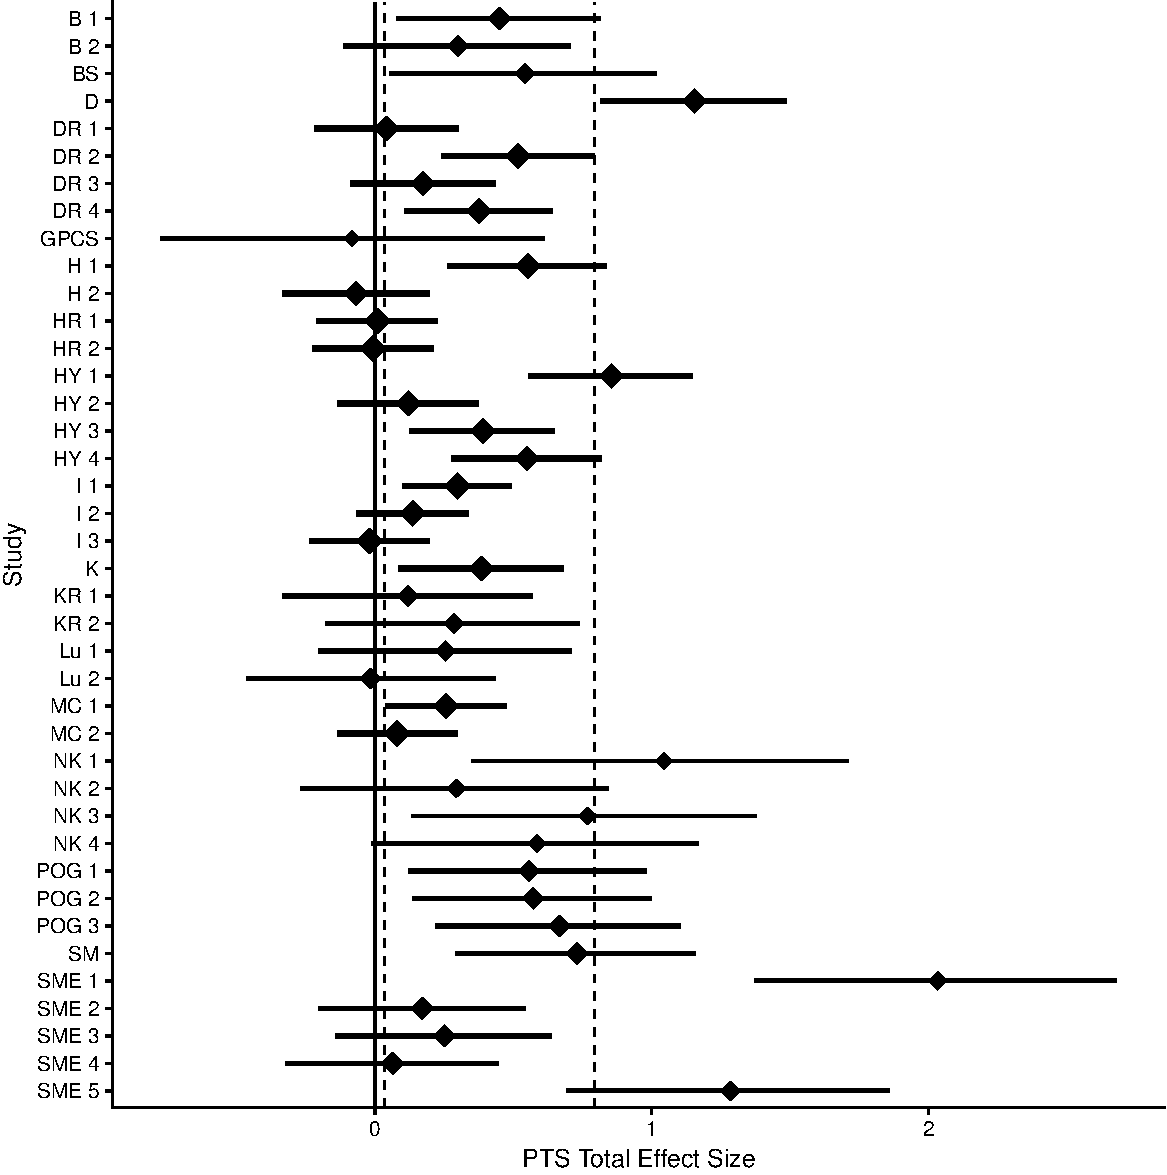
\includegraphics{meta_markdown_files/figure-latex/ptspicoverall-1.pdf}
\caption{\label{fig:ptspicoverall}Effect sizes and their non-centralized
confidence interval for PTS total scores. Dashed lines indicated average
non-weighted lower and upper confidence interval limits. Diamond size
indicates normalized study weight from a random effects model.}
\end{figure}

\begin{figure}[htbp]
\centering
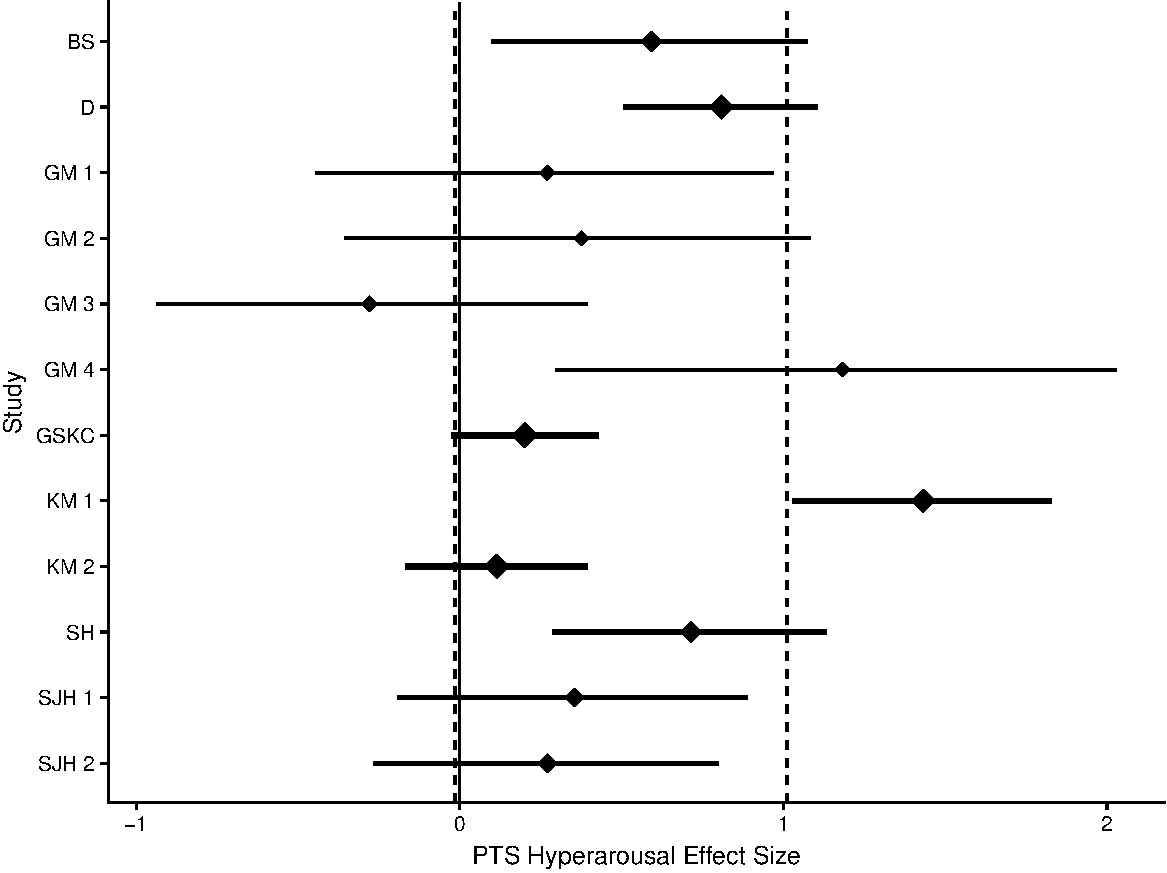
\includegraphics{meta_markdown_files/figure-latex/ptspichyper-1.pdf}
\caption{\label{fig:ptspichyper}Effect sizes and their non-centralized
confidence interval for PTS Hyperarousal. Dashed lines indicated average
non-weighted lower and upper confidence interval limits. Diamond size
indicates normalized study weight from a random effects model.}
\end{figure}

\begin{figure}[htbp]
\centering
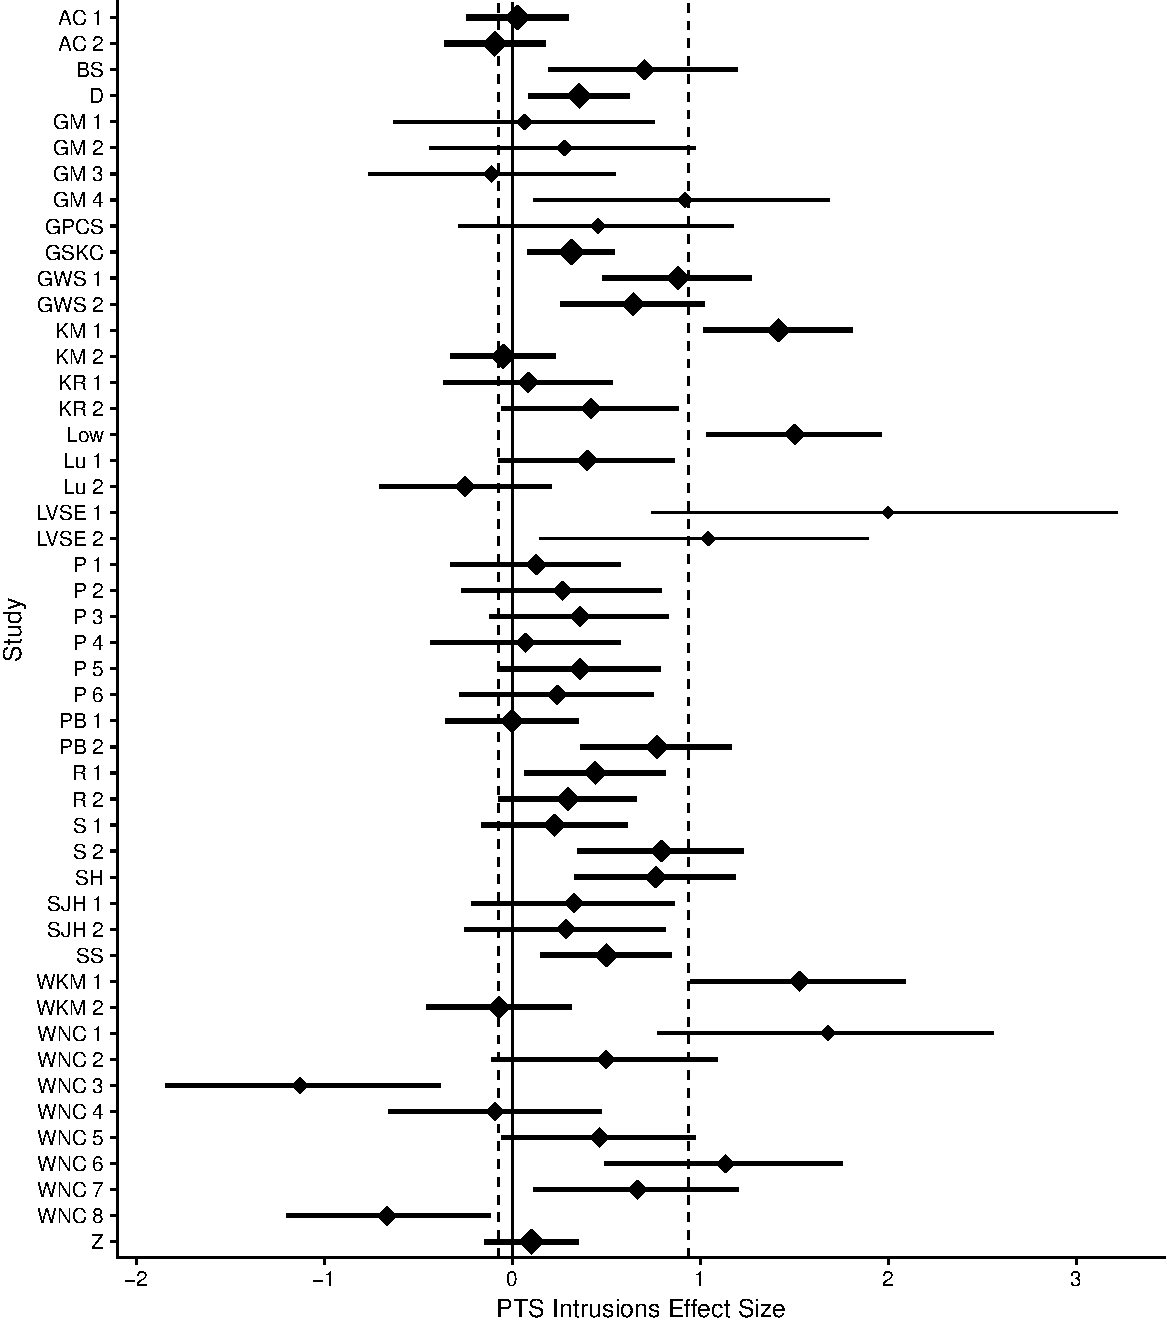
\includegraphics{meta_markdown_files/figure-latex/ptspicint-1.pdf}
\caption{\label{fig:ptspicint}Effect sizes and their non-centralized
confidence interval for PTS Intrusion scores. Dashed lines indicated
average non-weighted lower and upper confidence interval limits. Diamond
size indicates normalized study weight from a random effects model.}
\end{figure}

\begin{figure}[htbp]
\centering
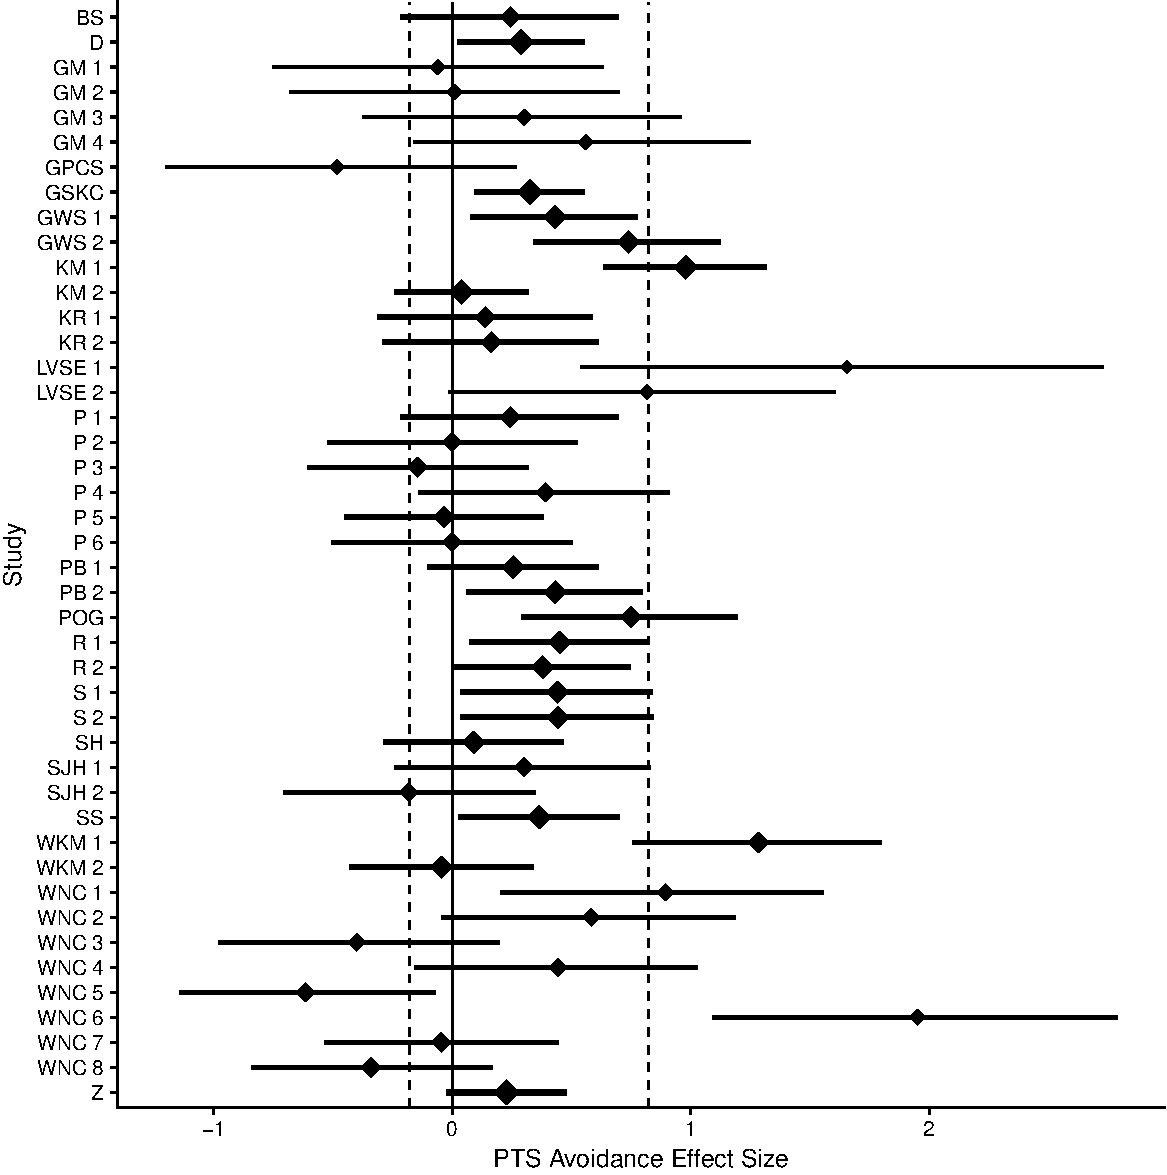
\includegraphics{meta_markdown_files/figure-latex/ptspicavoid-1.pdf}
\caption{\label{fig:ptspicavoid}Effect sizes and their non-centralized
confidence interval for PTS Avoidance Scores. Dashed lines indicated
average non-weighted lower and upper confidence interval limits. Diamond
size indicates normalized study weight from a random effects model.}
\end{figure}

\subsubsection{Homogeneity}\label{homogeneity}

A prerequisite for newer meta-analytic techniques includes the
assessment of homogeneity of the effects (Aert et al., 2016). Using the
\emph{metafor} package in \emph{R}, we calculated the \emph{Q}-statistic
and the \(I^2\) index (Cochran, 1954; Huedo-Medina, Sánchez-Meca,
Marín-Martínez, \& Botella, 2006). Significant values imply
inconsistencies across the variable or variables of interest and are
represented by \emph{Q}. In contrast, \(I^2\) indicates the percentage
of heterogeneity along with a 95\% CI. Both can, however, be biased with
a small number of experiments included for analyses (Higgins, Thompson,
Deeks, \& Altman, 2003; Huedo-Medina et al., 2006). Thus, we sought to
calculate an overall level of heterogeneity after examining each
variable separately before and after excluding outliers. For PTS studies
including outliers, we found significant heterogeneity, \emph{Q}(143) =
639.98, \emph{p} \textless{} .001 and \(I^2\) = 77.7, 95\% CI{[}73.9 -
80.9{]}. These values were reduced slightly with the exclusion of
outliers, \emph{Q}(140) = 519.75, \emph{p} \textless{} .001 and \(I^2\)
= 73.1, 95\% CI{[}68.2 - 77.2{]}.

\subsubsection{Power}\label{power}

Power was calculated in two different ways using the \emph{pwr} package
in \emph{R} (Champely, 2016). \emph{Post hoc} power was first calculated
using sample size and effect size statistics from each individual study.
Additionally, we calculated power using the study sample size and
estimated overall effect size from the random effects model with and
without outliers, as explained by G. Francis (2012) and G. Francis
(2014). The first estimate indicates the likelihood of finding an effect
from our sample statistics, while the second indicates the likelihood of
finding the true population effect size. If each study had been
conducted on only the change in the experimental group, 45.1\% of
studies would have been considered significant at \(\alpha\) \textless{}
.05. The average power of these studies based on their original study
characteristics was .46 (\emph{SD} = .36). Power for the random-effects
meta-analytic effect size with outliers was .47 (\emph{SD} = .24) and
without outliers was .42 (\emph{SD} = .23). Therefore, power
consistently was around 40-50\% for studies examining PTS, regardless of
outlier effects. In these studies, only 26.4\% achieved recommended 80\%
power for their found effect size, a smaller 16.7\% for the
random-effect outlier effect size, and even smaller 6.9\% for power
calculations on the random-effect size without the outliers.

\subsubsection{Other Meta-Analytic
Estimates}\label{other-meta-analytic-estimates}

As noted in Aert et al. (2016), \emph{p}-curve and \emph{p}-uniform
analyses are upwardly biased when heterogeneity is high. Therefore, we
use caution when interpreting these analyses on PTS outcomes. As seen in
Table \ref{tab:PTStable}, the estimates for \emph{p}-uniform were higher
than other techniques, likely because of the focus on significant
\emph{p}-values and the great degree of heterogeneity described earlier.
\emph{P}-curve pictures can be found at \url{https://osf.io/4mjqt/}
online, and this analysis indicated evidentiary value at \emph{p}
\textless{} .001. Additionally, the \emph{p}-uniform analysis indicated
that there was likely no publication bias present, \emph{Z} = -5.02,
\emph{p} = 1.000. When examining the PET analysis, we found that the
intercept was significant, which indicated that PEESE was likely a
better estimator of the meta-analytic effect size. PEESE estimates were
lower than the original meta-analytic estimate, but confidence intervals
indicated that the effect is small to medium, and still larger than
zero. Selection models indicated a larger effect size, especially with
the random-effects models, and these effects were influenced by the
outliers found in the published studies. Trim and fill models are shown
in Table \ref{tab:PTStable}, and figures are included online. Nineteen
missing studies were imputed for both models with and without outliers.
Across all these effect size estimates, we found that expressive writing
was likely to decrease PTS symptoms in a small to moderate way. The
correlation of effect size with time between measurement times was
\(r = -.16\), 95\% CI \([-.32\), \(.00]\), \(t(142) = -1.99\),
\(p = .049\), and \(r = -.15\), 95\% CI \([-.30\), \(.02]\),
\(t(139) = -1.75\), \(p = .082\) without outliers. This result indicated
that the effect of expressive writing slightly decreased across time.

\begin{table}[tbp]
\begin{center}
\begin{threeparttable}
\caption{\label{tab:PTStable}Effect Size Estimates for PTS Results}
\small{
\begin{tabular}{lcccc}
\toprule
Model & Fixed Effects & Random Effects & Fixed No Outliers & Random No Outliers\\
\midrule
Overall Effects & 0.34 [0.31, 0.37] & 0.39 [0.32, 0.46] & 0.32 [0.29, 0.35] & 0.36 [0.29, 0.42]\\
$Z$ Values & 21.75, $p$ < .001 & 11.06, $p$ < .001 & 20.00, $p$ < .001 & 11.03, $p$ < .001\\
$p$-Uniform & 0.60 [0.50, 0.71] & - & 0.57 [0.47, 0.67] & -\\
PET & 0.12 [0.03, 0.21] & - & 0.11 [0.02, 0.20] & -\\
PEESE & 0.25 [0.20, 0.30] & - & 0.23 [0.18, 0.28] & -\\
Selection Models & 0.33 [0.28, 0.37] & 0.45 [0.33, 0.57] & 0.29 [0.24, 0.33] & 0.39 [0.27, 0.50]\\
Trim and Fill & 0.26 [0.23, 0.29] & 0.26 [0.18, 0.34] & 0.25 [0.22, 0.28] & 0.25 [0.18, 0.32]\\
\bottomrule
\addlinespace
\end{tabular}
}
\begin{tablenotes}[para]
\textit{Note.} [] indicates the 95 percent confidence interval for each effect size estimate.
\end{tablenotes}
\end{threeparttable}
\end{center}
\end{table}

\subsection{PTG}\label{ptg}

\subsubsection{Overall Effect Size}\label{overall-effect-size-1}

Both fixed and random effects models with centralized confidence
intervals for PTG are presented in Table \ref{tab:PTGtable}. When
examining expressive writing on PTG, no outliers were detected. Fixed
and random effects estimates are included in Table \ref{tab:PTGtable},
while Figure \ref{fig:ptgpic} shows effect sizes for PTG studies where
shape size indicates the normalized weight of the study. Dashed lines
indicate non-weighted lower and upper confidence intervals for
non-centralized estimates. Overall, PTG studies indicated a negligible
to small effect size across both random and fixed effects models, and
the non-centralized confidence intervals indicated an effect that
crossed zero.

\begin{figure}[htbp]
\centering
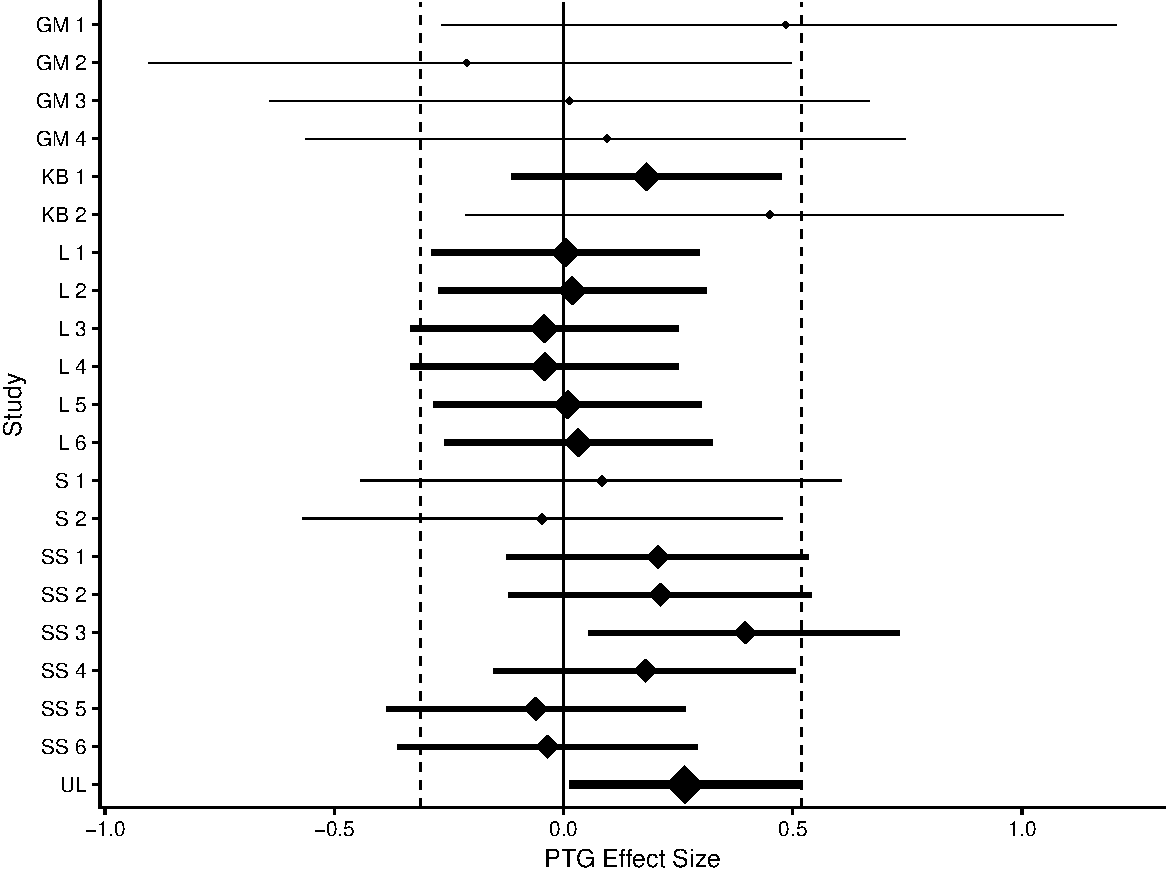
\includegraphics{meta_markdown_files/figure-latex/ptgpic-1.pdf}
\caption{\label{fig:ptgpic}Effect sizes and their non-centralized confidence
interval for PTG outcome variables. Dashed lines indicated average
non-weighted lower and upper confidence interval limits. Diamond size
indicates normalized study weight from a random effects model.}
\end{figure}

\subsubsection{Homogeneity}\label{homogeneity-1}

Using the \emph{metafor} package in \emph{R}, we calculated both a
\emph{Q} statistic and \(I^2\) index. Since PTG studied did not contain
any outliers, we did not calculate two separate analyses to examine
heterogeneity both with and without outliers. We did not find
significant heterogeneity across PTG studies, \emph{Q}(20) = 14.18,
\emph{p} = .82 and \(I^2\) = 0.0, 95\% CI{[}0.0 - 25.3{]}.

\subsubsection{Power}\label{power-1}

First, we calculated \emph{post hoc} power using both sample and effect
size statistics from individual studies. Individual studies examining
change in experimental groups showed that 9.5\% of studies would have
been considered significant at \(\alpha\) \textless{} .05. Average power
of PTG studies was .15 (\emph{SD} = .16). 0.0\% achieved recommended
80\% power for their found effect size. Additionally, we calculated
power using study sample size and estimated effect size from our random
effects model. Power for the true effect size was .08 (\emph{SD} = .02).
Again, 0.0\% achieved recommended 80\% power.

\subsubsection{Other Meta-Analytic
Estimates}\label{other-meta-analytic-estimates-1}

Due to no heterogeneity across PTG studies, we can use both
\emph{p}-curve and \emph{p}-uniform analyses with more confidence. A
pictorial representation of \emph{p}-curve can be found at
\url{https://osf.io/4mjqt/}. This analysis did not indicate evidentiary
value, \emph{p} = .75, as only two of the results would be considered
significant at \(\alpha\) \textless{} .05. \emph{p}-uniform estimates
are presented in Table \ref{tab:PTGtable}. Specifically, these analyses
indicated that there was no publication bias present, \emph{Z} = 0.70,
\emph{p} = .243. The \emph{p}-uniform estimates of the effect size for
PTG were negative, in contrast to the fixed and random effects overall
model. The confidence interval for this analysis indicates a wide range
of possible effects. In examining PET-PEESE analyses, we did not find a
significant intercept, indicating that PET is most likely a better
effect size estimator. PET analyses indicated that the effect size is
negligible to small, with our confidence interval crossing zero. These
results corroborated our original effect size calculations. Selection
models indicated negligible to small effect sizes, again wherein the
confidence interval includes zero effect. Trim and fill models are shown
in Table \ref{tab:PTGtable}, and figures are included online. Zero
studies were imputed for our model, and thus, the effect size estimate
is the same as the overall model. Across techniques, we found that
expressive writing has little to no effect on PTG. The correlation of
effect size across measurement times in PTG studies at subsequent time
points was \(r = .09\), 95\% CI \([-.36\), \(.50]\), \(t(19) = 0.38\),
\(p = .707\), and no change over time was found.

\begin{table}[tbp]
\begin{center}
\begin{threeparttable}
\caption{\label{tab:PTGtable}Effect Size Estimates for PTG Results}
\small{
\begin{tabular}{lcc}
\toprule
Model & Fixed Effects & Random Effects\\
\midrule
Overall Effects & 0.10 [0.02, 0.17] & 0.10 [0.02, 0.17]\\
$Z$ Values & 2.45, $p$ = .014 & 2.45, $p$ = .014\\
$p$-Uniform & -0.11 [-1.43, 0.42] & -\\
PET & 0.06 [-0.20, 0.32] & -\\
PEESE & 0.08 [-0.04, 0.20] & -\\
Selection Models & 0.09 [-0.01, 0.18] & 0.09 [-0.03, 0.20]\\
Trim and Fill & 0.10 [0.02, 0.17] & 0.10 [0.02, 0.17]\\
\bottomrule
\addlinespace
\end{tabular}
}
\begin{tablenotes}[para]
\textit{Note.} [] indicates the 95 percent confidence interval for each effect size estimate.
\end{tablenotes}
\end{threeparttable}
\end{center}
\end{table}

\subsection{QOL}\label{qol}

\subsubsection{Overall Effect Size}\label{overall-effect-size-2}

Finally, for QOL, both fixed and random effects models with centralized
confidence intervals are presented in Table \ref{tab:QOLtable}. Two
outliers were detected with this procedure, average \emph{d} = -0.07.
While the average effect of these outliers indicates a small number, it
is important to note that these two outliers were the largest positive
and negative effects found from the Possemato, Ouimette, and Geller
(2010) study. Fixed and random effects estimates without these points
are also included in Table \ref{tab:QOLtable}, while Figure
\ref{fig:qolpic} shows effect sizes for QOL studies. Overall, QOL
studies indicated a negligible to small effect that showed a
non-significant decrease in quality of life as a result of expressive
writing.

\begin{figure}[htbp]
\centering
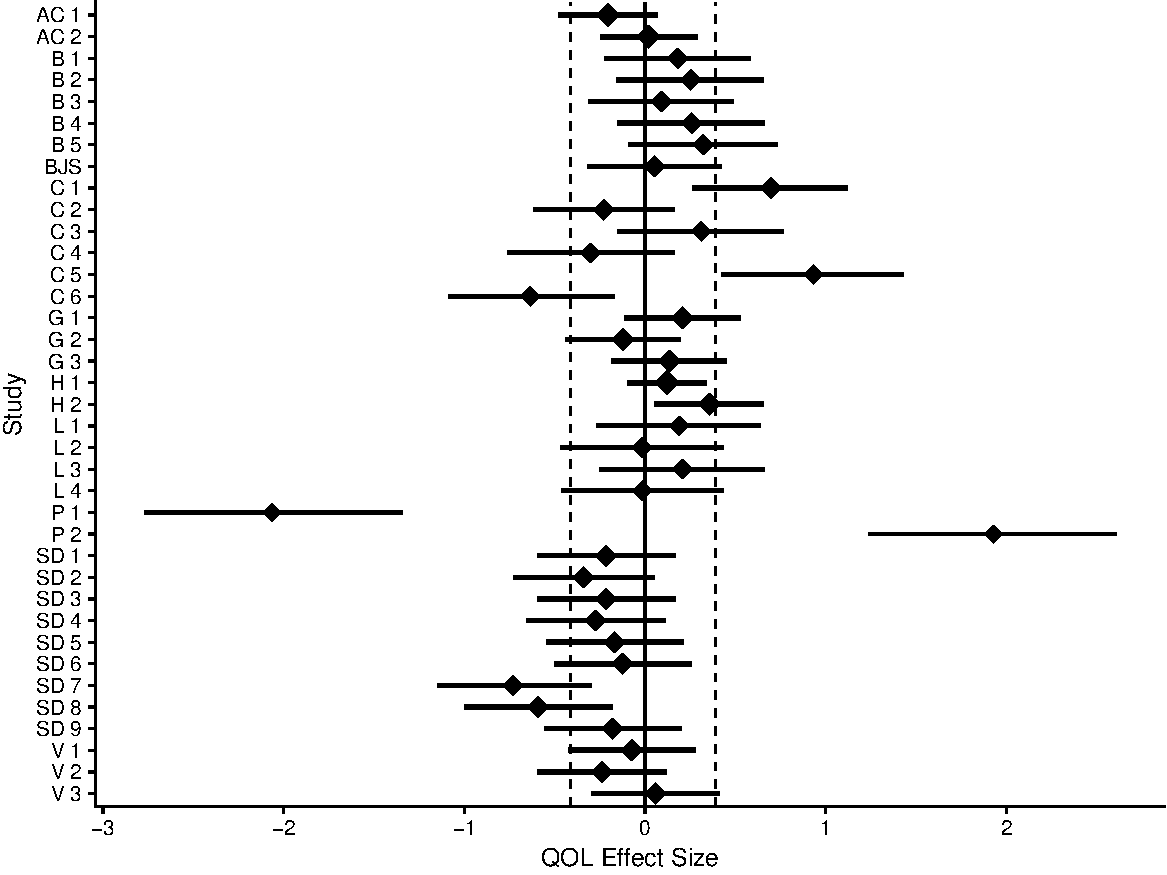
\includegraphics{meta_markdown_files/figure-latex/qolpic-1.pdf}
\caption{\label{fig:qolpic}Effect sizes and their non-centralized confidence
interval for QOL outcome variables. Dashed lines indicated average
non-weighted lower and upper confidence interval limits. Diamond size
indicates normalized study weight from a random effects model.}
\end{figure}

\subsubsection{Homogeneity}\label{homogeneity-2}

For QOL studies including outliers, we found significant heterogeneity
from our random effects model, \emph{Q}(36) = 200.09, \emph{p}
\textless{} .001 and \(I^2\) = 82.0, 95\% CI{[}75.9 - 86.5{]}. After
excluding outliers, our random effects model still indicated
heterogeneity,\emph{Q}(34) = 93.18, \emph{p} \textless{} .001 and
\(I^2\) = 63.5, 95\% CI{[}47.6 - 74.6{]}.

\subsubsection{Power}\label{power-2}

In conducting \emph{post hoc} power using sample and effect size
statistics from individual studies, we found that 21.6\% of studies
would have been considered significant at \(\alpha\) \textless{} .05.
Average power based on actual study characteristics was .33 (\emph{SD} =
.32). Power for the random effects meta-analytic effect size with
outliers was .05 (\emph{SD} = .00) and without outliers was .05
(\emph{SD} = .00). Unfortunately, power was around 5\% for both random
effects models with and without outliers. In these studies, 18.9\%
achieved adequate power of 80\% on their found effect size, while 0.0\%
achieved 80\% power for our random effects model with outliers. Finally,
without outliers, 0.0\% achieved 80\% power.

\subsubsection{Other Meta-Analytic
Estimates}\label{other-meta-analytic-estimates-2}

We exert caution in interpreting \emph{p}-curve and \emph{p}-uniform
analyses on QOL outcomes with and without outliers due to heterogeneity.
As seen in Table \ref{tab:PTStable}, \emph{p}-uniform estimates were
stronger and positive than other techniques because of the high degree
of heterogeneity recently described. \emph{p}-curve pictures can be
found at the following OSF Link: \url{https://osf.io/4mjqt}. Eight
studies were significant at \(\alpha\) \textless{} .05, and the studies
indicated evidentiary value, \emph{p} = .004. \emph{p}-uniform analyses
did not indicate publication bias, \emph{Z} = -2.75, \emph{p} = .997. In
PET-PEESE analyses, we found that the intercept was not significant, and
therefore, PET was a better estimator of the meta-analytic effect. Table
\ref{tab:PTStable} indicates that both of these analyses estimate the
effect size around zero, with a confidence interval that includes zero.
Selection models correspondingly show small effects crossing zero,
except for random effects models with outliers, that appear to be
heavily influenced by the outliers. Trim and fill models are shown in
Table \ref{tab:QOLtable}, and figures are included online. No studies
were imputed for these analyses, and therefore, the effect size
estimates match the original meta-analysis. Overall, these results
appear to point to no effects, ranging across zero with several negative
estimates. Interestingly, the correlation of effect sizes across
measurement times with outliers was \(r = -.37\), 95\% CI \([-.62\),
\(-.05]\), \(t(35) = -2.33\), \(p = .026\) and \(r = -.64\), 95\% CI
\([-.80\), \(-.39]\), \(t(33) = -4.75\), \(p < .001\) without outliers.
The effect of expressive writing appears to be positive at short time
intervals and decreases into negative effects at longer time intervals.

\begin{table}[tbp]
\begin{center}
\begin{threeparttable}
\caption{\label{tab:QOLtable}Effect Size Estimates for QOL Results}
\small{
\begin{tabular}{lcccc}
\toprule
Model & Fixed Effects & Random Effects & Fixed No Outliers & Random No Outliers\\
\midrule
Overall Effects & -0.01 [-0.07, 0.05] & -0.01 [-0.16, 0.13] & -0.01 [-0.07, 0.05] & -0.01 [-0.11, 0.09]\\
$Z$ Values & -0.33, $p$ = .745 & -0.18, $p$ = .860 & -0.25, $p$ = .805 & -0.20, $p$ = .838\\
$p$-Uniform & 0.79 [0.33, 1.61] & - & 0.62 [0.10, 0.96] & -\\
PET & 0.05 [-0.26, 0.36] & - & 0.05 [-0.29, 0.38] & -\\
PEESE & 0.00 [-0.17, 0.17] & - & 0.00 [-0.19, 0.19] & -\\
Selection Models & -0.06 [-0.12, 0.01] & 0.51 [-0.09, 1.12] & -0.04 [-0.11, 0.03] & 0.05 [-0.15, 0.24]\\
Trim and Fill & -0.01 [-0.07, 0.05] & -0.01 [-0.16, 0.13] & -0.01 [-0.07, 0.05] & -0.01 [-0.11, 0.09]\\
\bottomrule
\addlinespace
\end{tabular}
}
\begin{tablenotes}[para]
\textit{Note.} [] indicates the 95 percent confidence interval for each effect size estimate.
\end{tablenotes}
\end{threeparttable}
\end{center}
\end{table}

\section{Discussion}\label{discussion}

In examining pre- to post-test comparisons across each variable
separately, we found that PTS studies indicated a small effect size
across all meta-analytic estimates. Both QOL and PTG studies indicated a
negligible to small effect size using random effects models. Although
the PTG effect in our overall meta-analysis estimate was significant,
other methods indicate this small effect is likely not different from
zero. QOL was not different from zero, which suggests no effect of
expressive writing on quality of life. Interestingly, these results are
in contrast to Sloan et al. (2011), which suggested that only certain
groups may respond to these tasks. Potentially, the high heterogeneity
may be due to the mixed levels of PTSD in these studies, as Di Blasio et
al. (2015) indicates that only certain levels of PTSD are responsive to
an expressive writing condition.

Expressive writing does not appear to play an important role in
influencing positive growth or improved quality of life post task.
Ineffective emotional expression may be a contributing factor. In line
with this observation, the authors note several limitations. If
participants/clients are not deeply engaged with the material, an
expressive writing task may not be effective, as Pennebaker and Graybeal
(2001) imply that connectedness is an important factor for the task.
However, it may be difficult to implement a check for engagement in
these types of research designs. Doing so may also set a context that
will inhibit emotional processing and general responses. Research on
expressive writing has found a wide range of outcomes for different
variables (Frattaroli, 2006), and these various results may explain the
large heterogeneity found in this study. Encouragingly, we did not find
much evidence of publication bias, and therefore, these estimates may
represent a true population effect size. Regardless, methodology of
expressive writing studies is variable, as it is applied in different
forms across different contexts. Ideally, it would be possible to
control for these varied instructions and protocols. However, this is
simply not feasible, as most studies do not use measures that examine
how engaged an individual is with the material. As such, this current
meta-analysis sought to provide readers with a global effect of
expressive writing on the aforementioned outcome variables. More studies
are needed to examine potential moderating effects of participant
engagement.

We also examined the relationship of time between measurements of the
dependent variables and the corresponding effect size to determine if
effects change over time. For both PTS and PTG, there was no
relationship between effect size and time; yet, PTS indicated a small
negative correlation. This correlation was not, however, significant.
For QOL studies, a medium to large negative correlation was found. A
negative relationship between time and effect size implies that writing
tasks were more effective in the initial time points, and effects
decreased over longer time spans.

The psychological scientific community has shifted focus to
reproducibility and research design in the last several years (Nelson,
Simmons, \& Simonsohn, 2018), and much of this discussion has focused on
adequately powering studies for publication (Bakker et al., 2016; S. E.
Maxwell, Lau, \& Howard, 2015). S. E. Maxwell et al. (2015) and Open
Science Collaboration (2015) have shown that the \enquote{replication
crisis} may be attributed to low power in published studies. The power
found in the current meta-analysis was very poor, with very few studies
reaching the suggested 80\% criterion to adequately power their study.
This result was the same when considering individual study
characteristics or the estimate true population effect size. Research by
Bakker et al. (2016) indicates that researchers' intuitions about power
are particularly poor, and many studies could benefit from more informed
power analyses. Anderson, Kelley, and Maxwell (2017) recently published
a primer on power, with an online application to help with sample size
planning for many types of research designs. Additionally, we encourage
researchers to report power analyses of studies in order to better
understand methodology for replication and reproducibility.

Meta-analyses, while useful tools to pool for population effect sizes,
contain various limitations to their usefulness (Van Elk et al., 2015).
As mentioned previously, these analyses can be affected by high
heterogeneity, which was found in this study (Aert et al., 2016).
Selection models have been criticized when using a smaller number of
studies (Van Assen et al., 2015), and trim and fill analyses may not
always estimate accurate confidence intervals and funnel plots may be
biased with heterogeneity (Terrin, Schmid, Lau, \& Olkin, 2003). When
focusing on improving the psychological sciences, Van Elk et al. (2015)
suggest that the reliability and size of effects may be best elucidated
by conducting large preregistered studies. This suggestion will also
improve the outlook for power in published studies, and projects such as
Many Labs can aide in subsidizing large samples (R. A. Klein et al.,
2014). Even with limitations, meta-analyses allow researchers to examine
the state of a research area, and we find potential with expressive
writing on reducing PTS symptoms, and an overall need for better sample
size and power planning for studies.

\newpage

\section{References}\label{references}

\setlength{\parindent}{-0.5in} \setlength{\leftskip}{0.5in}

\hypertarget{refs}{}
\hypertarget{ref-VanAert2016}{}
Aert, R. C. M. van, Wicherts, J. M., \& Van Assen, M. A. L. M. (2016).
Conducting meta-analyses based on p-values: Reservations and
recommendations for applying p-uniform and p-curve. \emph{Perspectives
on Psychological Science}, \emph{11}(5), 713--729.
doi:\href{https://doi.org/10.1017/CBO9781107415324.004}{10.1017/CBO9781107415324.004}

\hypertarget{ref-AmericanPsychiatricAssociation2013}{}
American Psychiatric Association. (2013). \emph{Diagnostic and
statistical manual of mental disorders}.
doi:\href{https://doi.org/10.1176/appi.books.9780890425596.744053}{10.1176/appi.books.9780890425596.744053}

\hypertarget{ref-Anderson2017a}{}
Anderson, S. F., Kelley, K., \& Maxwell, S. E. (2017). Sample-size
planning for more accurate statistical power: A method adjusting sample
effect sizes for publication bias and uncertainty. \emph{Psychological
Science}, \emph{28}(11), 1547--1562.
doi:\href{https://doi.org/10.1177/0956797617723724}{10.1177/0956797617723724}

\hypertarget{ref-Aslam2013}{}
Aslam, N., \& Kamal, A. (2013). Gender differences in distress
responses, rumination patterns, perceived social support and
posttraumatic growth among flood affected individuals. \emph{Journal of
Pakistan Psychiatric Society}, \emph{10}, 86--90.

\hypertarget{ref-Bakker2016}{}
Bakker, M., Hartgerink, C. H. J., Wicherts, J. M., \& Maas, H. L. J. van
der. (2016). Researchers' intuitions about power in psychological
research. \emph{Psychological Science}, \emph{27}(8), 1069--1077.
doi:\href{https://doi.org/10.1177/0956797616647519}{10.1177/0956797616647519}

\hypertarget{ref-Bodor2002}{}
Bodor, N. Z. (2002). \emph{The health effects of emotional disclosure
for individuals with Type 1 diabetes} (PhD thesis No. 10-B). Retrieved
from
\href{http://ezproxy.lib.utexas.edu/login?url=http://search.ebscohost.com/login.aspx?direct=true\%7B/\&\%7Ddb=psyhref\%7B/\&\%7DAN=2006.20202.0010013}{http://ezproxy.lib.utexas.edu/login?url=http://search.ebscohost.com/login.aspx?direct=true\{\textbackslash{}\&\}db=psyhref\{\textbackslash{}\&\}AN=2006.20202.0010013}

\hypertarget{ref-Borenstein2007}{}
Borenstein, M., Hedges, L. V., \& Rothstein, H. (2007). Meta-analysis
fixed effect vs. random effects. Retrieved from
\href{https://www.meta-analysis.com/downloads/Meta-analysis\%20fixed\%20effect\%20vs\%20random\%20effects\%20072607.pdf}{https://www.meta-analysis.com/downloads/Meta-analysis fixed effect vs random effects 072607.pdf}

\hypertarget{ref-Brouneus2010}{}
Brounéus, K. (2010). The trauma of truth telling: Effects of witnessing
in the Rwandan Gacaca Courts on psychological health. \emph{Journal of
Conflict Resolution}, \emph{54}(3), 408--437.
doi:\href{https://doi.org/10.1177/0022002709360322}{10.1177/0022002709360322}

\hypertarget{ref-Bruns2016}{}
Bruns, S. B., \& Ioannidis, J. P. A. (2016). P-curve and p-hacking in
observational research. \emph{PLoS ONE}, \emph{11}(2).
doi:\href{https://doi.org/10.1371/journal.pone.0149144}{10.1371/journal.pone.0149144}

\hypertarget{ref-Buchanan2017}{}
Buchanan, E. M., Valentine, K. D., \& Scofield, J. E. (2017). MOTE.
Retrieved from \url{https://github.com/doomlab/MOTE}

\hypertarget{ref-Carter2014}{}
Carter, E. C., \& McCullough, M. E. (2014). Publication bias and the
limited strength model of self-control: Has the evidence for ego
depletion been overestimated? \emph{Frontiers in Psychology},
\emph{5}(July), 1--11.
doi:\href{https://doi.org/10.3389/fpsyg.2014.00823}{10.3389/fpsyg.2014.00823}

\hypertarget{ref-Champely2016}{}
Champely, S. (2016). pwr: Basic functions for power analysis. R package
version 1.2-0. Retrieved from
\url{https://cran.r-project.org/package=pwr}

\hypertarget{ref-Cobb2006}{}
Cobb, A. R., Tedeschi, R. G., Calhoun, L. G., \& Cann, A. (2006).
Correlates of posttraumatic growth in survivors of intimate partner
violence. \emph{Journal of Traumatic Stress}, \emph{19}(6), 895--903.
doi:\href{https://doi.org/10.1002/jts.20171}{10.1002/jts.20171}

\hypertarget{ref-Coburn2017}{}
Coburn, K. M., \& Vevea, J. L. (2017). Weightr. Retrieved from
\url{https://cran.r-project.org/web/packages/weightr/index.html}

\hypertarget{ref-Cochran1954}{}
Cochran, W. G. (1954). Some methods for strengthening the common
\(\chi\) 2 tests. \emph{Biometrics}, \emph{10}(4), 417--451.
doi:\href{https://doi.org/10.2307/3001616}{10.2307/3001616}

\hypertarget{ref-Cohen1988}{}
Cohen, J. (1988). \emph{Statistical power analysis for the behavioral
sciences} (2nd ed.). Hillsdale, NJ: Earlbaum.

\hypertarget{ref-Cooper2009}{}
Cooper, H., Hedges, L. V., \& Valentine, J. (2009). \emph{The handbook
of research synthesis and meta-analysis} (2nd ed.). New York, NY:
Russell Sage Foundation.

\hypertarget{ref-Costanza2007}{}
Costanza, R., Fisher, B., Ali, S., Beer, C., Bond, L., Boumans, R.,
\ldots{} Snapp, R. (2007). Quality of life: An approach integrating
opportunities, human needs, and subjective well-being. \emph{Ecological
Economics}, \emph{61}(2-3), 267--276.
doi:\href{https://doi.org/10.1016/j.ecolecon.2006.02.023}{10.1016/j.ecolecon.2006.02.023}

\hypertarget{ref-Crespo2016}{}
Crespo, M., \& Gomez, M. M. (2016). Diagnostic concordance of DSM-IV and
DSM-5 posttraumatic stress disorder (PTSD) in a clinical sample.
\emph{Psicothema}, \emph{28}(2), 161--166.
doi:\href{https://doi.org/10.7334/psicothema2015.213}{10.7334/psicothema2015.213}

\hypertarget{ref-Cumming2012}{}
Cumming, G. (2012). \emph{Understanding the new statistics: Effect
sizes, confidence intervals, and meta-analysis}. New York, NY:
Routledge.

\hypertarget{ref-DerSimonian1986}{}
DerSimonian, R., \& Laird, N. (1986). Meta-analysis in clinical trials.
\emph{Controlled Clinical Trials}, \emph{7}(3), 177--188.
doi:\href{https://doi.org/10.1016/0197-2456(86)90046-2}{10.1016/0197-2456(86)90046-2}

\hypertarget{ref-Blasio2015a}{}
Di Blasio, P., Camisasca, E., Caravita, S. C. S., Ionio, C., Milani, L.,
Valtolina, G. G., \ldots{} Valtolina, G. G. (2015). The effects of
expressive writing on postpartum depression and posttraumatic stress
symptoms. \emph{Psychological Reports}, \emph{117}(3), 856--882.
doi:\href{https://doi.org/10.2466/02.13.PR0.117c29z3}{10.2466/02.13.PR0.117c29z3}

\hypertarget{ref-Dursun2016}{}
Dursun, P., Steger, M. F., Bentele, C., \& Schulenberg, S. E. (2016).
Meaning and posttraumatic growth among survivors of the September 2013
Colorado floods. \emph{Journal of Clinical Psychology}, \emph{72}(12),
1247--1263.
doi:\href{https://doi.org/10.1002/jclp.22344}{10.1002/jclp.22344}

\hypertarget{ref-Duval2000}{}
Duval, S., \& Tweedie, R. (2000). Trim and fill: A simple
funnel-plot-based method of testing and adjusting for publication bias
in meta-analysis. \emph{Biometrics}, \emph{56}(2), 455--463.
doi:\href{https://doi.org/10.1111/j.0006-341X.2000.00455.x}{10.1111/j.0006-341X.2000.00455.x}

\hypertarget{ref-Egger1997}{}
Egger, M., Davey Smith, G., Schneider, M., \& Minder, C. (1997). Bias in
meta-analysis detected by a simple, graphical test. \emph{British
Medical Journal}, \emph{315}(7109), 629--634.
doi:\href{https://doi.org/10.1136/bmj.316.7129.469}{10.1136/bmj.316.7129.469}

\hypertarget{ref-Esterling1990}{}
Esterling, B. A., Antoni, M. H., Kumar, M., \& Schneiderman, N. (1990).
Emotional repression, stress disclosure responses, and Epstein-Barr
viral capsid antigen titers. \emph{Psychosomatic Medicine}, \emph{52},
397--410.
doi:\href{https://doi.org/10.1097/00006842-199007000-00002}{10.1097/00006842-199007000-00002}

\hypertarget{ref-Fawzy1993}{}
Fawzy, N. W., Fawzy, N. W., Hyun, C. S., Elashoff, R., Guthrie, D.,
Fahey, J. L., \& Morton, D. L. (1993). Malignant melanoma. Effects of an
early structured psychiatric intervention, coping, and affective state
on recurrence and survival 6 years later. \emph{Archives of General
Psychiatry}, \emph{50}(9), 681--689.
doi:\href{https://doi.org/10.1001/archpsyc.1993.01820210015002}{10.1001/archpsyc.1993.01820210015002}

\hypertarget{ref-Francis2012}{}
Francis, G. (2012). Publication bias and the failure of replication in
experimental psychology. \emph{Psychonomic Bulletin \& Review},
\emph{19}(6), 975--991.
doi:\href{https://doi.org/10.3758/s13423-012-0322-y}{10.3758/s13423-012-0322-y}

\hypertarget{ref-Francis2014}{}
Francis, G. (2014). The frequency of excess success for articles in
Psychological Science. \emph{Psychonomic Bulletin \& Review},
\emph{21}(5), 1180--1187.
doi:\href{https://doi.org/10.3758/s13423-014-0601-x}{10.3758/s13423-014-0601-x}

\hypertarget{ref-Francis1992}{}
Francis, M. E., \& Pennebaker, J. W. (1992). Putting stress into words:
The impact of writing on physiological, absentee, and self-reported
emotional well-being measures. \emph{American Journal of Health
Promotion}, \emph{6}(4), 280--287.
doi:\href{https://doi.org/10.4278/0890-1171-6.4.280}{10.4278/0890-1171-6.4.280}

\hypertarget{ref-Frankl1959}{}
Frankl, V. (1959). \emph{Man's search for meaning} (3rd ed.). Boston,
MA: Beacon Press.

\hypertarget{ref-Frattaroli2006}{}
Frattaroli, J. (2006). Experimental disclosure and its moderators: A
meta-analysis. \emph{Psychological Bulletin}, \emph{132}(6), 823--865.
doi:\href{https://doi.org/10.1037/0033-2909.132.6.823}{10.1037/0033-2909.132.6.823}

\hypertarget{ref-Frisina2004a}{}
Frisina, P. G., Borod, J. C., \& Lepore, S. J. (2004). A meta-analysis
of the effects of written emotional disclosure on the health outcomes of
clinical populations. \emph{The Journal of Nervous and Mental Disease},
\emph{192}(9), 629--634.
doi:\href{https://doi.org/10.1097/01.nmd.0000138317.30764.63}{10.1097/01.nmd.0000138317.30764.63}

\hypertarget{ref-Gentes2014}{}
Gentes, E. L., Dennis, P. A., Kimbrel, N. A., Rissling, M. B., Beckham,
J. C., \& Calhoun, P. S. (2014). DSM-5 posttraumatic stress disorder:
Factor structure and rates of diagnosis. \emph{Journal of Psychiatric
Research}, \emph{59}(1), 60--67.
doi:\href{https://doi.org/10.1016/j.jpsychires.2014.08.014}{10.1016/j.jpsychires.2014.08.014}

\hypertarget{ref-Gidron1996a}{}
Gidron, Y., Peri, T., Connolly, J. F., \& Shalev, A. Y. (1996). Written
disclosure in posttraumatic stress disorder: Is it beneficial for the
patient? \emph{The Journal of Nervous and Mental Disease},
\emph{184}(8), 505--506.
doi:\href{https://doi.org/10.1097/00005053-199608000-00009}{10.1097/00005053-199608000-00009}

\hypertarget{ref-Glass1976}{}
Glass, G. V. (1976). Primary, secondary, and meta-analysis of research.
\emph{Educational Researcher}, \emph{5}(10), 3--8.
doi:\href{https://doi.org/10.3102/0013189X005010003}{10.3102/0013189X005010003}

\hypertarget{ref-Goldstein1988}{}
Goldstein, H. S., Edelberg, R., Meier, C. F., \& Davis, L. (1988).
Relationship of resting blood pressure and heart rate to experienced
anger and expressed anger. \emph{Psychosomatic Medicine}, \emph{50}(4),
321--329.
doi:\href{https://doi.org/10.1097/00006842-198807000-00001}{10.1097/00006842-198807000-00001}

\hypertarget{ref-Greenberg1992}{}
Greenberg, M. A., \& Stone, A. A. (1992). Emotional disclosure about
traumas and its relation to health: Effects of previous disclosure and
trauma severity. \emph{Journal of Personality and Social Psychology},
\emph{63}, 75--84.
doi:\href{https://doi.org/10.1037/h0090372}{10.1037/h0090372}

\hypertarget{ref-Gross1997}{}
Gross, J. J., \& Levenson, R. W. (1997). Hiding feelings: The acute
effects of inhibiting negative and positive emotion. \emph{Journal of
Abnormal Psychology}, \emph{106}(1), 95--103.
doi:\href{https://doi.org/10.1037/0021-843X.106.1.95}{10.1037/0021-843X.106.1.95}

\hypertarget{ref-Harris2005}{}
Harris, A. H. S., Thoresen, C. E., Humphreys, K., \& Faul, J. (2005).
Does writing affect asthma? A randomized trial. \emph{Psychosomatic
Medicine}, \emph{67}(1), 130--136.
doi:\href{https://doi.org/10.1097/01.psy.0000146345.73510.d5}{10.1097/01.psy.0000146345.73510.d5}

\hypertarget{ref-Hedges1982}{}
Hedges, L. V. (1982). Estimation of effect size from a series of
independent experiments. \emph{Psychological Bulletin}, \emph{92}(2),
490--499.
doi:\href{https://doi.org/10.1037/0033-2909.92.2.490}{10.1037/0033-2909.92.2.490}

\hypertarget{ref-Henry2010}{}
Henry, E. A., Schlegel, R. J., Talley, A. E., Molix, L. A., \&
Bettencourt, B. A. (2010). The feasibility and effectiveness of
expressive writing for rural and urban breast cancer survivors.
\emph{Oncology Nursing Forum}, \emph{37}(6), 749--757.
doi:\href{https://doi.org/10.1188/10.ONF.749-757}{10.1188/10.ONF.749-757}

\hypertarget{ref-Higgins2003}{}
Higgins, J. P. T., Thompson, S. G., Deeks, J. J., \& Altman, D. G.
(2003). Measuring inconsistency in meta-analyses. \emph{British Medical
Journal}, \emph{327}(7414), 557--560.
doi:\href{https://doi.org/10.1136/bmj.327.7414.557}{10.1136/bmj.327.7414.557}

\hypertarget{ref-Hilgard2016}{}
Hilgard, J. (2016). PETPEESE. GitHub. Retrieved from
\url{https://github.com/Joe-Hilgard/PETPEESE}

\hypertarget{ref-Huedo-Medina2006}{}
Huedo-Medina, T. B., Sánchez-Meca, J., Marín-Martínez, F., \& Botella,
J. (2006). Assessing heterogeneity in meta-analysis: Q statistic or I²
index? \emph{Psychological Methods}, \emph{11}(2), 193--206.
doi:\href{https://doi.org/10.1037/1082-989X.11.2.193}{10.1037/1082-989X.11.2.193}

\hypertarget{ref-John2012}{}
John, L. K., Loewenstein, G., \& Prelec, D. (2012). Measuring the
prevalence of questionable research practices with incentives for truth
telling. \emph{Psychological Science}, \emph{23}(5), 524--532.
doi:\href{https://doi.org/10.1177/0956797611430953}{10.1177/0956797611430953}

\hypertarget{ref-Kelley2007}{}
Kelley, K. (2007). Confidence intervals for standardized effect sizes.
\emph{Journal of Statistical Software}, \emph{20}(8), 1--24.
doi:\href{https://doi.org/10.18637/jss.v020.i08}{10.18637/jss.v020.i08}

\hypertarget{ref-Klein2014a}{}
Klein, R. A., Ratliff, K. A., Vianello, M., Adams, R. B., Bahník, Š.,
Bernstein, M. J., \ldots{} Nosek, B. A. (2014). Investigating variation
in replicability. \emph{Social Psychology}, \emph{45}(3), 142--152.
doi:\href{https://doi.org/10.1027/1864-9335/a000178}{10.1027/1864-9335/a000178}

\hypertarget{ref-Klump2008}{}
Klump, M. C. (2008). Posttraumatic stress disorder and sexual assault in
women. \emph{Journal of College Student Development}, \emph{8225}(May
2014), 37--41.
doi:\href{https://doi.org/10.1300/J035v21n02}{10.1300/J035v21n02}

\hypertarget{ref-Kross2011}{}
Kross, E., \& Ayduk, O. (2011). Making meaning out of negative
experiences by self-distancing. \emph{Current Directions in
Psychological Science}, \emph{20}(3), 187--191.
doi:\href{https://doi.org/10.1177/0963721411408883}{10.1177/0963721411408883}

\hypertarget{ref-Lakens2013}{}
Lakens, D. (2013). Calculating and reporting effect sizes to facilitate
cumulative science: A practical primer for t-tests and ANOVAs.
\emph{Frontiers in Psychology}, \emph{4}.
doi:\href{https://doi.org/10.3389/fpsyg.2013.00863}{10.3389/fpsyg.2013.00863}

\hypertarget{ref-Lancaster2015}{}
Lancaster, S. L., Klein, K. P., \& Heifner, A. (2015). The validity of
self-reported growth after expressive writing. \emph{Traumatology},
\emph{21}(4), 293--298.
doi:\href{https://doi.org/10.1037/trm0000052}{10.1037/trm0000052}

\hypertarget{ref-Larson1990a}{}
Larson, D. G., \& Chastain, R. L. (1990). Self-concealment:
Conceptualization, measurement, and health implications. \emph{Journal
of Social and Clinical Psychology}, \emph{9}(4), 439--455.
doi:\href{https://doi.org/10.1521/jscp.1990.9.4.439}{10.1521/jscp.1990.9.4.439}

\hypertarget{ref-Lieberman2006}{}
Lieberman, M. A., \& Goldstein, B. A. (2006). Not all negative emotions
are equal: The role of emotional expression in online support groups for
women with breast cancer. \emph{Psycho-Oncology}, \emph{15}(2),
160--168. doi:\href{https://doi.org/10.1002/pon.932}{10.1002/pon.932}

\hypertarget{ref-Maxwell2015}{}
Maxwell, S. E., Lau, M. Y., \& Howard, G. S. (2015). Is psychology
suffering from a replication crisis? What does ``failure to replicate''
really mean? \emph{American Psychologist}, \emph{70}(6), 487--498.
doi:\href{https://doi.org/10.1037/a0039400}{10.1037/a0039400}

\hypertarget{ref-McShane2016}{}
McShane, B. B., Böckenholt, U., \& Hansen, K. T. (2016). Adjusting for
publication bias in meta-analysis. \emph{Perspectives on Psychological
Science}, \emph{11}(5), 730--749.
doi:\href{https://doi.org/10.1177/1745691616662243}{10.1177/1745691616662243}

\hypertarget{ref-Meshberg-Cohen2014}{}
Meshberg-Cohen, S., Svikis, D., \& McMahon, T. J. (2014). Expressive
writing as a therapeutic process for drug-dependent women.
\emph{Substance Abuse}, \emph{35}(1), 80--88.
doi:\href{https://doi.org/10.1080/08897077.2013.805181}{10.1080/08897077.2013.805181}

\hypertarget{ref-Mogk2006}{}
Mogk, C., Otte, S., Reinhold-Hurley, B., \& Kröner-Herwig, B. (2006).
Health effects of expressive writing on stressful or traumatic
experiences - a meta-analysis. \emph{Psychosocial Medicine}, \emph{3},
Doc06.

\hypertarget{ref-Morris2002}{}
Morris, S. B., \& DeShon, R. P. (2002). Combining effect size estimates
in meta-analysis with repeated measures and independent-groups designs.
\emph{Psychological Methods}, \emph{7}(1), 105--125.
doi:\href{https://doi.org/10.1037/1082-989X.7.1.105}{10.1037/1082-989X.7.1.105}

\hypertarget{ref-Nelson2018}{}
Nelson, L. D., Simmons, J., \& Simonsohn, U. (2018). Psychology's
renaissance. \emph{Annual Review of Psychology}, \emph{69}(1), 511--534.
doi:\href{https://doi.org/10.1146/annurev-psych-122216-011836}{10.1146/annurev-psych-122216-011836}

\hypertarget{ref-OpenScienceCollaboration2015}{}
Open Science Collaboration. (2015). Estimating the reproducibility of
psychological science. \emph{Science}, \emph{349}(6251),
aac4716--aac4716.
doi:\href{https://doi.org/10.1126/science.aac4716}{10.1126/science.aac4716}

\hypertarget{ref-Pennebaker1989}{}
Pennebaker, J. W. (1989). Confession, inhibition, and disease. In L.
Berkowitz (Ed.), \emph{Advances in experimental social psychology} (Vol.
22, pp. 211--244). Academic Press.
doi:\href{https://doi.org/10.1016/S0065-2601(08)60309-3}{10.1016/S0065-2601(08)60309-3}

\hypertarget{ref-Pennebaker1993}{}
Pennebaker, J. W. (1993). Putting stress into words: Health, linguistic,
and therapeutic implications. \emph{Behaviour Research and Therapy},
\emph{31}(6), 539--548.
doi:\href{https://doi.org/10.1016/0005-7967(93)90105-4}{10.1016/0005-7967(93)90105-4}

\hypertarget{ref-Pennebaker1986}{}
Pennebaker, J. W., \& Beall, S. K. (1986). Confronting a traumatic
event: Toward an understanding of inhibition and disease. \emph{Journal
of Abnormal Psychology}, \emph{95}(3), 274--281.
doi:\href{https://doi.org/10.1037//0021-843X.95.3.274}{10.1037//0021-843X.95.3.274}

\hypertarget{ref-Pennebaker1996}{}
Pennebaker, J. W., \& Francis, M. E. (1996). Cognitive, emotional, and
language processes in disclosure. \emph{Cognition \& Emotion},
\emph{10}(6), 601--626.
doi:\href{https://doi.org/10.1080/026999396380079}{10.1080/026999396380079}

\hypertarget{ref-Pennebaker2001}{}
Pennebaker, J. W., \& Graybeal, A. (2001). Patterns of natural language
use: Disclosure, personality, and social integration. \emph{Current
Directions in Psychological Science}, \emph{10}(3), 90--93.
doi:\href{https://doi.org/10.1111/1467-8721.00123}{10.1111/1467-8721.00123}

\hypertarget{ref-Pennebaker1990}{}
Pennebaker, J. W., Colder, M., \& Sharp, L. K. (1990). Accelerating the
coping process. \emph{Journal of Personality and Social Psychology},
\emph{58}(3), 528--537.
doi:\href{https://doi.org/10.1037//0022-3514.58.3.528}{10.1037//0022-3514.58.3.528}

\hypertarget{ref-Pennebaker1988}{}
Pennebaker, J. W., Kiecolt-Glaser, J. K., \& Glaser, R. (1988).
Disclosure of traumas and immune function: Health implications for
psychotherapy. \emph{Journal of Consulting and Clinical Psychology},
\emph{56}(2), 239--245.
doi:\href{https://doi.org/10.1037/0022-006X.56.2.239}{10.1037/0022-006X.56.2.239}

\hypertarget{ref-Possemato2010}{}
Possemato, K., Ouimette, P., \& Geller, P. (2010). Internet-based
expressive writing for kidney transplant recipients: Effects on
posttraumatic stress and quality of life. \emph{Traumatology},
\emph{16}(1), 49--54.
doi:\href{https://doi.org/10.1177/1534765609347545}{10.1177/1534765609347545}

\hypertarget{ref-Rachman1980}{}
Rachman, S. (1980). Emotional processing. \emph{Behaviour Research and
Therapy}, \emph{18}(1), 51--60.
doi:\href{https://doi.org/10.1016/0005-7967(80)90069-8}{10.1016/0005-7967(80)90069-8}

\hypertarget{ref-Reinhold2018}{}
Reinhold, M., Bürkner, P. C., \& Holling, H. (2018). Effects of
expressive writing on depressive symptoms---A meta-analysis.
\emph{Clinical Psychology: Science and Practice}, \emph{25}(1).
doi:\href{https://doi.org/10.1111/cpsp.12224}{10.1111/cpsp.12224}

\hypertarget{ref-Sanchez-Meca2008a}{}
Sánchez-Meca, J., \& Marín-Martínez, F. (2008). Confidence intervals for
the overall effect size in random-effects meta-analysis.
\emph{Psychological Methods}, \emph{13}(1), 31--48.
doi:\href{https://doi.org/10.1037/1082-989X.13.1.31}{10.1037/1082-989X.13.1.31}

\hypertarget{ref-Scheff1979}{}
Scheff, T. J. (1979). \emph{Catharsis in healing, ritual, and drama}.
Los Angeles: University of California Press.

\hypertarget{ref-Schoutrop2002}{}
Schoutrop, M. J. A., Lange, A., Hanewald, G., Davidovich, U., \&
Salomon, H. H. (2002). Structured writing and processing major stressful
events: A controlled trial. \emph{Psychotherapy and Psychosomatics},
\emph{71}(3), 151--157.
doi:\href{https://doi.org/10.1159/000056282}{10.1159/000056282}

\hypertarget{ref-Schulenberg2008}{}
Schulenberg, S. E., Hutzell, R. R., Nassif, C., \& Rogina, J. M. (2008).
Logotherapy for clinical practice. \emph{Psychotherapy}, \emph{45}(4),
447--463. doi:\href{https://doi.org/10.1037/a0014331}{10.1037/a0014331}

\hypertarget{ref-Simonsohn2014}{}
Simonsohn, U., Nelson, L. D., \& Simmons, J. P. (2014). p-curve: A key
to the file-drawer. \emph{Journal of Experimental Psychology: General},
\emph{143}(2), 534--547.
doi:\href{https://doi.org/10.1037/a0033242}{10.1037/a0033242}

\hypertarget{ref-Simonsohn2015}{}
Simonsohn, U., Simmons, J. P., \& Nelson, L. D. (2015). Better p-curves:
Making p-curve analysis more robust to errors, fraud, and ambitious
p-hacking, a reply to Ulrich and Miller (2015). \emph{Journal of
Experimental Psychology: General}, \emph{144}(6), 1146--1152.
doi:\href{https://doi.org/10.1037/xge0000104}{10.1037/xge0000104}

\hypertarget{ref-Slavin-Spenny2011}{}
Slavin-Spenny, O. M., Cohen, J. L., Oberleitner, L. M., \& Lumley, M. A.
(2011). The effects of different methods of emotional disclosure:
Differentiating posttraumatic growth from stress symptoms. \emph{Journal
of Clinical Psychology}, \emph{67}(10), 993--1007.
doi:\href{https://doi.org/10.1002/jclp.20750}{10.1002/jclp.20750}

\hypertarget{ref-Sloan2005}{}
Sloan, D. M., Marx, B. P., \& Epstein, E. M. (2005). Further examination
of the exposure model underlying the efficacy of written emotional
disclosure. \emph{Journal of Consulting and Clinical Psychology},
\emph{73}(3), 549--554.
doi:\href{https://doi.org/10.1037/0022-006X.73.3.549}{10.1037/0022-006X.73.3.549}

\hypertarget{ref-Sloan2011a}{}
Sloan, D. M., Marx, B. P., \& Greenberg, E. M. (2011). A test of written
emotional disclosure as an intervention for posttraumatic stress
disorder. \emph{Behaviour Research and Therapy}, \emph{49}(4), 299--304.
doi:\href{https://doi.org/10.1016/j.brat.2011.02.001}{10.1016/j.brat.2011.02.001}

\hypertarget{ref-Sloan2012}{}
Sloan, D. M., Marx, B. P., Bovin, M. J., Feinstein, B. A., \& Gallagher,
M. W. (2012). Written exposure as an intervention for PTSD: A randomized
clinical trial with motor vehicle accident survivors. \emph{Behaviour
Research and Therapy}, \emph{50}(10), 627--635.
doi:\href{https://doi.org/10.1016/j.brat.2012.07.001}{10.1016/j.brat.2012.07.001}

\hypertarget{ref-Sloan2007}{}
Sloan, D. M., Marx, B. P., Epstein, E. M., \& Lexington, J. M. (2007).
Does altering the writing instructions influence outcome associated with
written disclosure? \emph{Behavior Therapy}, \emph{38}(2), 155--168.
doi:\href{https://doi.org/10.1016/j.beth.2006.06.005}{10.1016/j.beth.2006.06.005}

\hypertarget{ref-Smithson2001}{}
Smithson, M. (2001). Correct confidence intervals for various regression
effect sizes and parameters: The importance of noncentral distributions
in computing intervals. \emph{Educational and Psychological
Measurement}, \emph{61}(4), 605--632.
doi:\href{https://doi.org/10.1177/00131640121971392}{10.1177/00131640121971392}

\hypertarget{ref-Smithson2003}{}
Smithson, M. (2003). \emph{Confidence intervals}. Thousand Oaks, CA:
Sage.

\hypertarget{ref-Smyth1998}{}
Smyth, J. M. (1998). Written emotional expression: Effect sizes ,
outcome types, and moderating variables. \emph{Journal of Consulting and
Clinical Psychology}, \emph{66}(1), 174--184.
doi:\href{https://doi.org/10.1037/0022-006X.66.1.174}{10.1037/0022-006X.66.1.174}

\hypertarget{ref-Smyth1999}{}
Smyth, J. M., Stone, A. A., Hurewitz, A., \& Kaell, A. (1999). Effects
of writing about stressful experiences on symptom reduction in patients
with asthma or rheumatoid arthritis: A randomized trial. \emph{JAMA: The
Journal of the American Medical Association}, \emph{281}(14),
1304--1309.
doi:\href{https://doi.org/10.1001/jama.281.14.1304}{10.1001/jama.281.14.1304}

\hypertarget{ref-Stanley2005}{}
Stanley, T. D. (2005). Beyond publication bias. \emph{Journal of
Economic Surveys}, \emph{19}(3), 309--345.
doi:\href{https://doi.org/10.1111/j.0950-0804.2005.00250.x}{10.1111/j.0950-0804.2005.00250.x}

\hypertarget{ref-Stanley2014}{}
Stanley, T. D., \& Doucouliagos, H. (2014). Meta-regression
approximations to reduce publication selection bias. \emph{Research
Synthesis Methods}, \emph{5}(1), 60--78.
doi:\href{https://doi.org/10.1002/jrsm.1095}{10.1002/jrsm.1095}

\hypertarget{ref-Stanton2002}{}
Stanton, A. L., Danoff-Burg, S., Sworowski, L. A., Collins, C. A.,
Branstetter, A. D., Rodriguez-Hanley, A., \ldots{} Austenfeld, J. L.
(2002). Randomized, controlled trial of written emotional expression and
benefit finding in breast cancer patients. \emph{Journal of Clinical
Oncology}, \emph{20}(20), 4160--4168.
doi:\href{https://doi.org/10.1200/JCO.2002.08.521}{10.1200/JCO.2002.08.521}

\hypertarget{ref-Taku2008}{}
Taku, K., Calhoun, L. G., Cann, A., \& Tedeschi, R. G. (2008). The role
of rumination in the coexistence of distress and posttraumatic growth
among bereaved Japanese University students. \emph{Death Studies},
\emph{32}(5), 428--444.
doi:\href{https://doi.org/10.1080/07481180801974745}{10.1080/07481180801974745}

\hypertarget{ref-Tedeschi1995}{}
Tedeschi, R. G., \& Calhoun, L. G. (1995). \emph{Trauma \&
transformation: Growing in the aftermath of suffering.} Thousand Oaks,
CA: Sage Publications.

\hypertarget{ref-Tedeschi2004}{}
Tedeschi, R. G., \& Calhoun, L. G. (2004). Posttraumatic growth:
Conceptual foundations and empirical evidence. \emph{Psychological
Inquiry}, \emph{15}(1), 1--18.
doi:\href{https://doi.org/10.1207/s15327965pli1501}{10.1207/s15327965pli1501}

\hypertarget{ref-Terrin2003}{}
Terrin, N., Schmid, C. H., Lau, J., \& Olkin, I. (2003). Adjusting for
publication bias in the presence of heterogeneity. \emph{Statistics in
Medicine}, \emph{22}(13), 2113--2126.
doi:\href{https://doi.org/10.1002/sim.1461}{10.1002/sim.1461}

\hypertarget{ref-Theofilou2013}{}
Theofilou, P. (2013). Quality of life: Definition and measurement.
\emph{Europe's Journal of Psychology}, \emph{9}(1), 150--162.
doi:\href{https://doi.org/10.5964/ejop.v9i1.337}{10.5964/ejop.v9i1.337}

\hypertarget{ref-VanAert2017}{}
Van Aert, R. C. M. (2017). P-uniform. GitHub. Retrieved from
\url{https://github.com/RobbievanAert/puniform}

\hypertarget{ref-VanAssen2015}{}
Van Assen, M. A. L. M., Van Aert, R. C. M., \& Wicherts, J. M. (2015).
Meta-analysis using effect size distributions of only statistically
significant studies. \emph{Psychological Methods}, \emph{20}(3),
293--309.
doi:\href{https://doi.org/http://dx.doi.org/10.1037/met0000025}{http://dx.doi.org/10.1037/met0000025}

\hypertarget{ref-VanElk2015}{}
Van Elk, M., Matzke, D., Gronau, Q. F., Guan, M., Vandekerckhove, J., \&
Wagenmakers, E.-J. (2015). Meta-analyses are no substitute for
registered replications: A skeptical perspective on religious priming.
\emph{Frontiers in Psychology}, \emph{6}, 1365.
doi:\href{https://doi.org/10.3389/fpsyg.2015.01365}{10.3389/fpsyg.2015.01365}

\hypertarget{ref-VanEmmerik2013}{}
Van Emmerik, A. A. P., Reijntjes, A., \& Kamphuis, J. H. (2013). Writing
therapy for posttraumatic stress: A meta-analysis. \emph{Psychotherapy
and Psychosomatics}, \emph{82}(2), 82--88.
doi:\href{https://doi.org/10.1159/000343131}{10.1159/000343131}

\hypertarget{ref-Vevea1995}{}
Vevea, J. L., \& Hedges, L. V. (1995). A general linear model for
estimating effect size in the presence of publication bias.
\emph{Psychometrika}, \emph{60}(3), 419--435.
doi:\href{https://doi.org/10.1007/BF02294384}{10.1007/BF02294384}

\hypertarget{ref-Vevea2005}{}
Vevea, J. L., \& Woods, C. M. (2005). Publication bias in research
synthesis: Sensitivity analysis using a priori weight functions.
\emph{Psychological Methods}, \emph{10}(4), 428--443.
doi:\href{https://doi.org/10.1037/1082-989X.10.4.428}{10.1037/1082-989X.10.4.428}

\hypertarget{ref-Viechtbauer2010}{}
Viechtbauer, W. (2010). Conducting meta-analyses in R with the metafor
package. \emph{Journal of Statistical Software}, \emph{36}(3), 1--48.
doi:\href{https://doi.org/10.18637/jss.v036.i03}{10.18637/jss.v036.i03}

\hypertarget{ref-Walker1999a}{}
Walker, B. L., Nail, L. M., \& Croyle, R. T. (1999). Does emotional
expression make a difference in reactions to breast cancer?
\emph{Oncology Nursing Forum}, \emph{26}(6), 1025--1032.

\hypertarget{ref-Wang2000}{}
Wang, X., Gao, L., Shinfuku, N., Zhang, H., Zhao, C., \& Shen, Y.
(2000). Longitudinal study of earthquake-related PTSD in a randomly
selected community sample in North China. \emph{American Journal of
Psychiatry}, \emph{157}(8), 1260--1266.
doi:\href{https://doi.org/10.1176/appi.ajp.157.8.1260}{10.1176/appi.ajp.157.8.1260}

\hypertarget{ref-Weiss2002}{}
Weiss, T. (2002). Posttraumatic growth in women with breast cancer and
their husbands -- An intersubjective validation study. \emph{Journal of
Psychosocial Oncology}, \emph{20}(2), 65--80.
doi:\href{https://doi.org/10.1300/J077v20n02_04}{10.1300/J077v20n02\_04}

\hypertarget{ref-Wilson2009}{}
Wilson, K. G., \& DuFrene, T. (2009). \emph{Mindfulness for two: An
acceptance and commitment Therapy approach to mindfulness in
psychotherapy}. Oakland, CA: New Harbinger Publications.

\hypertarget{ref-Yilmaz2016}{}
Yilmaz, M., \& Zara, A. (2016). Traumatic loss and posttraumatic growth:
The effect of traumatic loss related factors on posttraumatic growth.
\emph{Anatolian Journal of Psychiatry}, \emph{17}(1), 5--11.
doi:\href{https://doi.org/10.5455/apd.188311}{10.5455/apd.188311}






\end{document}
